%=================================================================================
\chapter{Implementation in SWIFT}\label{chap:meshless-implementation}
%=================================================================================


To conclude the part on finite volume particle methods, their implementation in the cosmological
hydrodynamics code \swift \citep{schallerSWIFTUsingTaskbased2016,
schallerSWIFTSPHInterdependent2018a} is presented. It is fully open-source and publicly available on \url{https://gitlab.cosma.dur.ac.uk/swift/swiftsim} and on github under
\url{https://github.com/SWIFTSIM/swiftsim}, along with extensive documentation and a plethora of
ready-to-run examples.

\swift uses particles as the fundamental discretization elements, and has several flavors of
Smoothed Particle Hydrodynamics methods implemented. Gravity is solved using a fast multipole method \citep{chengFastAdaptiveMultipole1999, dehnenFastMultipoleMethod2014f} coupled to a particle mesh solver in Fourier space to deal with periodic volumes. In addition, several galaxy formation models are already implemented, most notably \codename{Eagle} \citep{schayeEAGLEProjectSimulating2015} and \codename{Gear} \citep{revazDynamicalChemicalEvolution2012}.

\swift is highly parallelized and makes use of a hybrid task-based parallelism strategy for shared
memory parallelism combined with MPI for distributed memory parallelism. The task-based parallelism
furthermore permits to exploit asynchronous MPI communications and a domain decomposition strategy
based on the work rather than data to efficiently utilize modern high performance computing
architectures. These technical aspects will be discussed in more detail in the subsequent sections,
as they are intimately tied to the manner in which the finite volume particle methods for the Euler
equations (and for the equations of radiative transfer in Part~\ref{part:rt}) need to be
implemented.









%----------------------------------------------------
\section{Task Based Parallelism}
%----------------------------------------------------

\begin{figure}
 \centering
 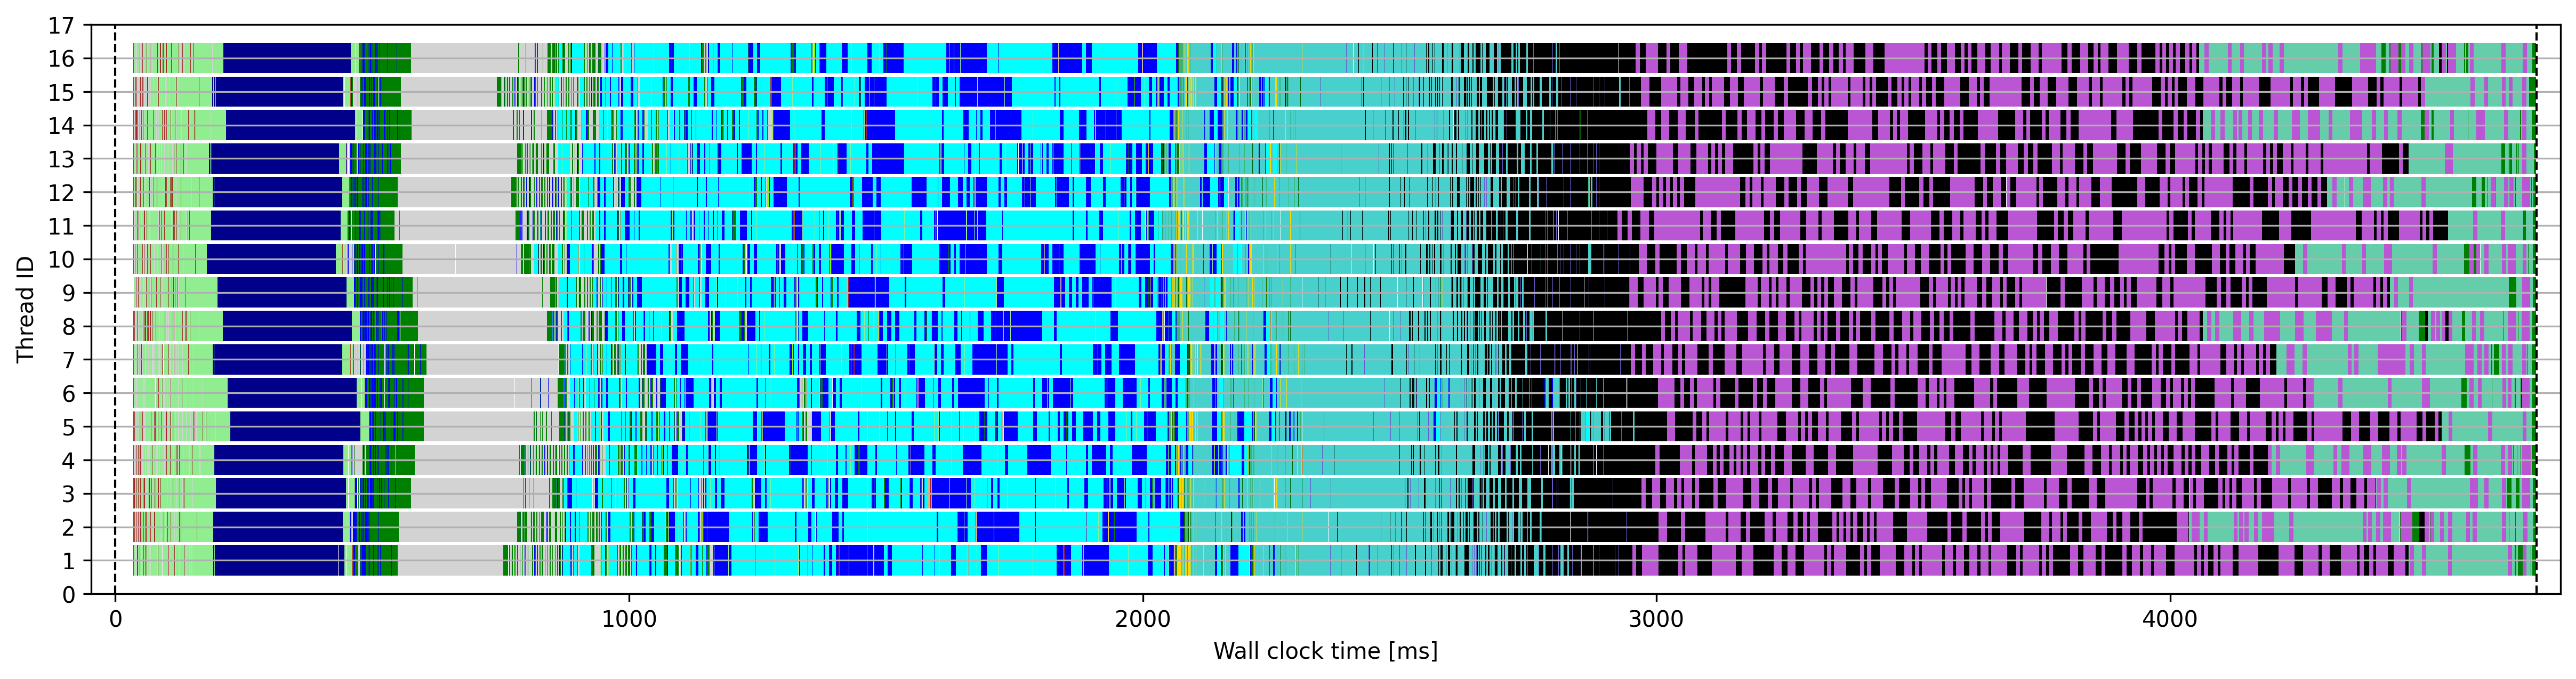
\includegraphics[width=\textwidth]{figures/Meshless/taskplot.png}%
 \caption{
One time step of a simulation using \swift with 16 threads. The colored blocks represent various
tasks being solved. Each color represents a different task type. Note how there is no noteworthy
idle time (white blocks) and how the varying threads are solving different types of tasks
concurrently, and that all threads finish at nearly the identical time.
 }
 \label{fig:taskplot}
\end{figure}

\swift relies on a task-based parallelism scheme
\citep{gonnetSWIFTFastAlgorithms2013, gonnetQuickSchedTaskbasedParallelism2016b,
theunsSWIFTTaskbasedHydrodynamics2015}.
The task-based parallelism is a system in which a full computation is divided into a set of
individual however inter-dependent tasks. They are dynamically allocated to idle cores by a
dedicated task scheduler \citep{gonnetQuickSchedTaskbasedParallelism2016b}.
%This strategy leads to
%both the automatic optimization of the load balancing as well as to the improvement of cache
%efficiency.
To illustrate the idea, consider the following scenario: ``\textit{If a construction worker requires
two weeks to pave a street, how long would it take ten construction workers?}'' In this analogy, the
paving of the street is the simulation that needs to be executed, while the construction workers are
computing cores.

In traditional parallelism schemes, every worker would execute the same sequence of tasks and
commands. Each construction worker would first clean up the place where the street needs to be
paved, then heat up their own portion of asphalt, pour it into place assigned for this worker, and
finally stomp the new asphalt in with a roller. Obviously employing more workers should lead to
finishing the job quicker, but there is room for improvement. For example, what if not all workers
can be assigned the same amount of street surface to work on? All workers that finished their share
of the job already would stand by idly waiting for the last one to complete their part. Having
workers just stand around with nothing to do is obviously a scenario we'd like to prevent.

This is one of the reasons why \swift (and other state-of-the-art codes like
\cite{stoneAthenaAdaptiveMesh2020}, \cite{wadsleyGasoline2ModernSmoothed2017},
\cite{menonAdaptiveTechniquesClustered2015})  moved towards a task-based parallelism scheme. This
means that instead of giving every worker exactly the same sequence of steps to do, we keep track of
all the individual jobs that need to be completed: Each section of the street needs to be cleaned
up, each section of the street requires its respective amount of asphalt heated up, then poured,
then rolled. Some of these jobs however can be completed concurrently: While some workers can clean
up the street, others can already start to heat up the asphalt. Once a section of the street is
cleaned up, the first asphalt can be poured. Simultaneously other workers can keep cleaning other
sections of the street and heating up more asphalt. This concurrent work is of prime interest for
the task-based parallelism scheme: As long as there is work to do, the workers shouldn't be idling.
To illustrate how the application of task-based parallelism can look like, Figure~\ref{fig:taskplot}
shows the tasks being executed during one time step of a simulation with \swift. The simulation was
run using 16 threads, and Figure~\ref{fig:taskplot} shows what each thread was working on during the
time step and how long it took. Different types of tasks are colored differently, and it clearly
shows how the varying threads are solving different types of tasks concurrently. Note how there is
no noteworthy idle time (white blocks) once the tasks start being executed and how all threads
finish at nearly the identical time.


This approach however requires us not only to define tasks, i.e. portions of work that a single
worker at a time could do, but also \emph{dependencies}. Some things need to be finished first
before others can be done: For example, one couldn't pour the asphalt before it's hot, nor could one
stomp it in before it's poured. Additionally, we need to also define \emph{conflicts}. Conflicts
between tasks arise in cases where there is work to be done for which the order of execution
doesn't matter, but it can't be done concurrently. This can for example be the case when two tasks
need to access and modify the same data, while the order of the access and modification is
unimportant. In the ``workers paving a road'' analogy, this could for example be the case when the
workers are finishing for the day and packing up their tools into their trucks. It doesn't really
matter which tools go in first, but only one tool can be put in the trunk at a time.

Task-based parallelism offers many benefits aside from reducing idle waiting time of CPUs. It can
be used to drastically decrease the times CPUs spend to fetch data from memory by ensuring that
tasks which act on a set of data are always executed by the same CPU. This way the memory remains
local, and the cache efficiency is increased. Furthermore, when dealing with distributed memory
architectures the tasks can be used as an adequate measure of the actual work that needs to be
performed. The domain decomposition between the nodes can then be performed based on sharing the
work equally rather than some proxy for the work like the number of cells or particles contained
within a region. Having other work available for threads to execute also enables \swift to use
asynchronous messages on distributed memory architectures: The threads don't need to perform
blocking messages, where both the sending and the receiving side do nothing but wait for each other
to complete the communication. Instead, the thread on the sending side can send the message and
continue doing other work, while the thread on the receiving side can start with the work once it's
notified that the message has been received and keep itself busy otherwise until the message
arrives.


However, task based parallelism also comes with several caveats. Firstly, it requires for tasks to
be generated during a simulation, and then for the scheduler to execute them, which constitutes
additional overhead work that needs to be done so the actual physics can be solved. The overhead is
noticeable for small problems, e.g. simulations that can be executed on a personal computer. With
increased problem size however, the benefits of the task-based parallelism make the overheads
negligible and lead to a significantly improved performance and scaling of the code in comparison
with traditional parallelization techniques (\cite{borrowSWIFTMaintainingWeakscalability2018}).
Secondly, the manual definition of tasks, dependencies, and conflicts necessary for the task-based
parallelization requires a considerable effort on the developing side. It doesn't suffice to write
code that solves the equations that govern the physics any longer. The entire framework of the
tasks, dependencies, and conflicts needs to be constructed first. The major difficulties with that
work is to identify and fix errors in the dependency logic. These difficulties arise because (a)
errors can be very hard to spot, since in real applications they manifest in certain variables being
accessed too early or too late without any warning, and (b) even when spotted, in general they
aren't reproducible because the execution order of the tasks is not fixed and may depend on
uncontrollable circumstances, e.g. which processing cores one gets access to for a given run, where
exactly in memory the processors need to fetch data from and how long that will take, etc. Matters
become even worse when distributed memory parallelization is included, as that adds an entire other
layer of unpredictability and irreproducibility.








%----------------------------------------------------------------------------------------------
\section[FVPM In \swift: Task Dependency Graph]{Hydrodynamics With Finite Volume Particle Methods
in SWIFT: Constructing the Task Dependency Graph}\label{chap:swift-hydro-tasks}
%----------------------------------------------------------------------------------------------

In this section, the tasks and dependencies required for the solution of hydrodynamics problems
using the finite volume particle methods in \swift is described. To begin with, let's remind
ourselves of the order of operations necessary for the finite volume particle hydrodynamics (see
Section~\ref{chap:meshless-full}), shown in Figure~\ref{fig:meshless-order-of-operations}. This
order of operations describes the order of work that needs to be done for each particle. In case
other physics are involved, in particular gravity, a second kick operation before the drift is
necessary for the integration to be sufficiently accurate. In what follows, we include that second
kick. The steps with a blue background, namely the neighbor search, the computation of gradients,
and the exchange of fluxes, are the steps that involve loops over neighboring particles.


\begin{figure}[H]
\centering
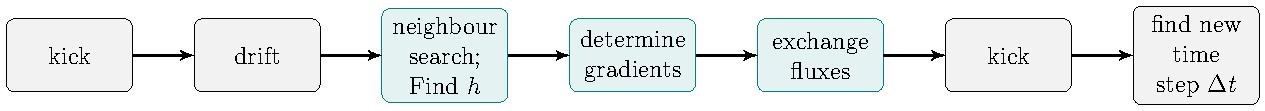
\includegraphics[width=\linewidth]{figures/Meshless/meshless_order_of_operations.pdf}%
\caption{The order of operations for a single time step required for the finite volume particle
methods for each particle using a kick-drift-kick time integration scheme. The steps with a blue
background, namely the neighbor search, the computation of gradients, and the exchange of fluxes,
are the steps that involve loops over neighboring particles.}
\label{fig:meshless-order-of-operations}
\end{figure}





%---------------------------------------------------
\subsection{Constructing Tasks}
%---------------------------------------------------

%---------------------------------------------------
\subsubsection{Grouping Particles in Cells}
%---------------------------------------------------

To develop the tasks and dependencies required for this order of operations to be executed on each
particle, we need to look into how the tasks and the particles are intertwined first.
As described in Section~\ref{chap:meshless-full}, a major component of the finite volume particle
schemes are the interactions between neighboring particles, and in particular the neighbor search
which is necessary each step. For the sake of optimization and quick access, particles are grouped
into cells whose size is determined by requiring that all neighbors of the particles within a cell
must be inside adjacent cells. This ensures that the number of adjacent cells that need to be
involved in an interaction are always known and predictable. Initially, the entire simulation domain
is divided into cells of equal size, called the ``\lingo{top level}'' cells. These \lingo{top
level} cells are then recursively split into cells with half the parent cell's size as much as
possible while the condition to have all neighbors of particles in adjacent cells is satisfied.
Having cells as small as possible and containing as few particles as possible is desirable as it
speeds up the neighbor search significantly by increasing the ratio of particles which are actually
neighbors of another particle to the number of total particles checked during the interactions.
However, we still
need to ensure that \emph{all} neighbors can be found in neighboring cells, which gives the lower
boundary of the cell size.





%-------------------------------------------------------------------
\subsubsection{Connecting Work and Data: Task Classes and Types}
%-------------------------------------------------------------------

Tasks are then attached to the cells, not the individual particles inside the cells. This means that
when a task is being executed, it operates on all the particles contained within a cell. At this
point, it's useful to begin differentiating between two classes of tasks. The first class would be
all the tasks which include interactions between particles, e.g. the neighbor search. Let's call
them ``\lingo{interaction}'' tasks. The other class of tasks conducts work exclusively on individual
particles, for example the drift and kick operations. The construction of these ``\lingo{plain}''
tasks is straightforward: All they need to do is go over all particles contained in a given cell to
which the task is attached to and do whatever it is set up to do on the particles individually. The
\lingo{interaction} tasks however are a little more contrived. They can again be split into two
different types of interactions. The first type, called ``\lingo{self}'' tasks, perform the
interactions of particles contained within a cell with all the other particles \emph{inside the same
cell}. \lingo{Self}-type tasks are always attached to a singe cell. The second type,
``\lingo{pair}'' tasks, perform the interactions of particles contained within a cell with the
particles contained within some neighboring cell. \lingo{Pair}-type tasks are always attached to a
pair of cells. The cells involved in the interaction are then always adjacent cells by construction.
Figure~\ref{fig:self-pair-tasks} illustrates the interactions involved with \lingo{self}- and
\lingo{pair}-type tasks. However, since cells are being split recursively into smaller ones until
they reach a lower limit, this means that not all leaf cells will have the same size, i.e. be at the
same level, and the tree structure of cells will have varying depths depending on the number of
particles currently situated there. This would mean that in some cases a task would need to interact
with cells of different sizes, and hence a variable number of \lingo{pair} type tasks needs to be
constructed between a cell and its potentially smaller sized adjacent cells. Rather than
constructing an individual task for each \lingo{pair} type interaction that might be necessary, we
pick some convenient cell level in the cell tree that we call the ``\lingo{super level}''.
All the tasks are then constructed and attached to cells at the \lingo{super level} in the tree.
The \lingo{super level} may or may not be the \lingo{top level}, i.e. the root of the cell tree. If
a \lingo{super level} cell is split and thus has children, \lingo{self}- and \lingo{pair}-tasks are
replaced by ``\lingo{sub-self}'' and ``\lingo{sub-pair}'' tasks which recursively descend to the
leaf cell level and perform all required interactions. Since each cell is split into eight children
cells of half the parent cell's dimensions, the recursion of a \lingo{sub-self} type tasks involves
calling a \lingo{sub-self} type task for each child cell as well as a \lingo{sub-pair} type task
for each pair of two child cells, such that all possible interactions are covered. The
\lingo{sub-pair} task recursion is handled analogously.


\begin{figure}
 \centering
 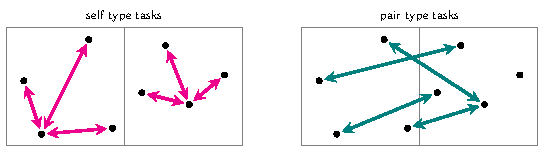
\includegraphics[width=\linewidth]{figures/Meshless/self-pair.pdf}%
 \caption{
 Two adjacent cells containing some particles are shown. On the left, the interactions of
\lingo{self} type tasks are illustrated: They only interact particles with other particles that
share a cell with them. On the right, \lingo{pair} type tasks are shown. They only interact
particles form one cell with the particles from the other cell. Some interactions between particles
have not been drawn for clarity, but in principle for \lingo{self}-type tasks all particles within
a cell will interact with all other particles in that cell. Similarly all particles of a cell
should interact with all particles in the neighboring cell in \lingo{pair}-type tasks. }
 \label{fig:self-pair-tasks}
\end{figure}




%---------------------------------------
\subsection{A First Dependency Graph}
%---------------------------------------

Using the \lingo{plain} and \lingo{interaction} classes of tasks, we can now begin to construct the
dependency graph that executes the correct order of operations for the finite volume particle
hydrodynamics scheme. In a first approach, the dependency graph will look like the order of
operations shown previously: The drift, kick, and timestep tasks will be \lingo{plain} tasks, while
the neighbor search, the gradient, and the flux exchange tasks will be \lingo{interaction} type
tasks, i.e. will be \lingo{self}, \lingo{sub-self}, \lingo{pair}, and \lingo{sub-pair} type tasks.
The tasks and dependencies can be represented by a directed acyclic graph, where the nodes are the
tasks, and the edges are the dependencies. A simplified dependency graph based only on the required
order of operations is shown in Figure~\ref{fig:dependency-graph-zeroth-order}. For completeness,
the full kick-drift-kick integration scheme is shown, and hence two kick tasks are included. The
task names are slightly changed to the convention used for smooth particle hydrodynamics:

\begin{itemize}
\item the tasks that drift the particles are called ``\lingo{drift\_part}''
\item the neighbor search interactions are called ``\lingo{density}'' tasks following the SPH
convention, as the neighbor search determines the particle densities.
\item \lingo{self}, \lingo{pair}, \lingo{sub-self}, and \lingo{sub-pair} type tasks are marked as
such with the corresponding prefix. E.g. the sub-self neighbor search interaction task is called
``\lingo{sub\_self\_density}''.
\item the flux exchange interactions are called ``\lingo{force}'' tasks following
the SPH convention again, as the second interaction loop in SPH evaluates the forces between
particles.
\end{itemize}


\begin{figure}
\centering
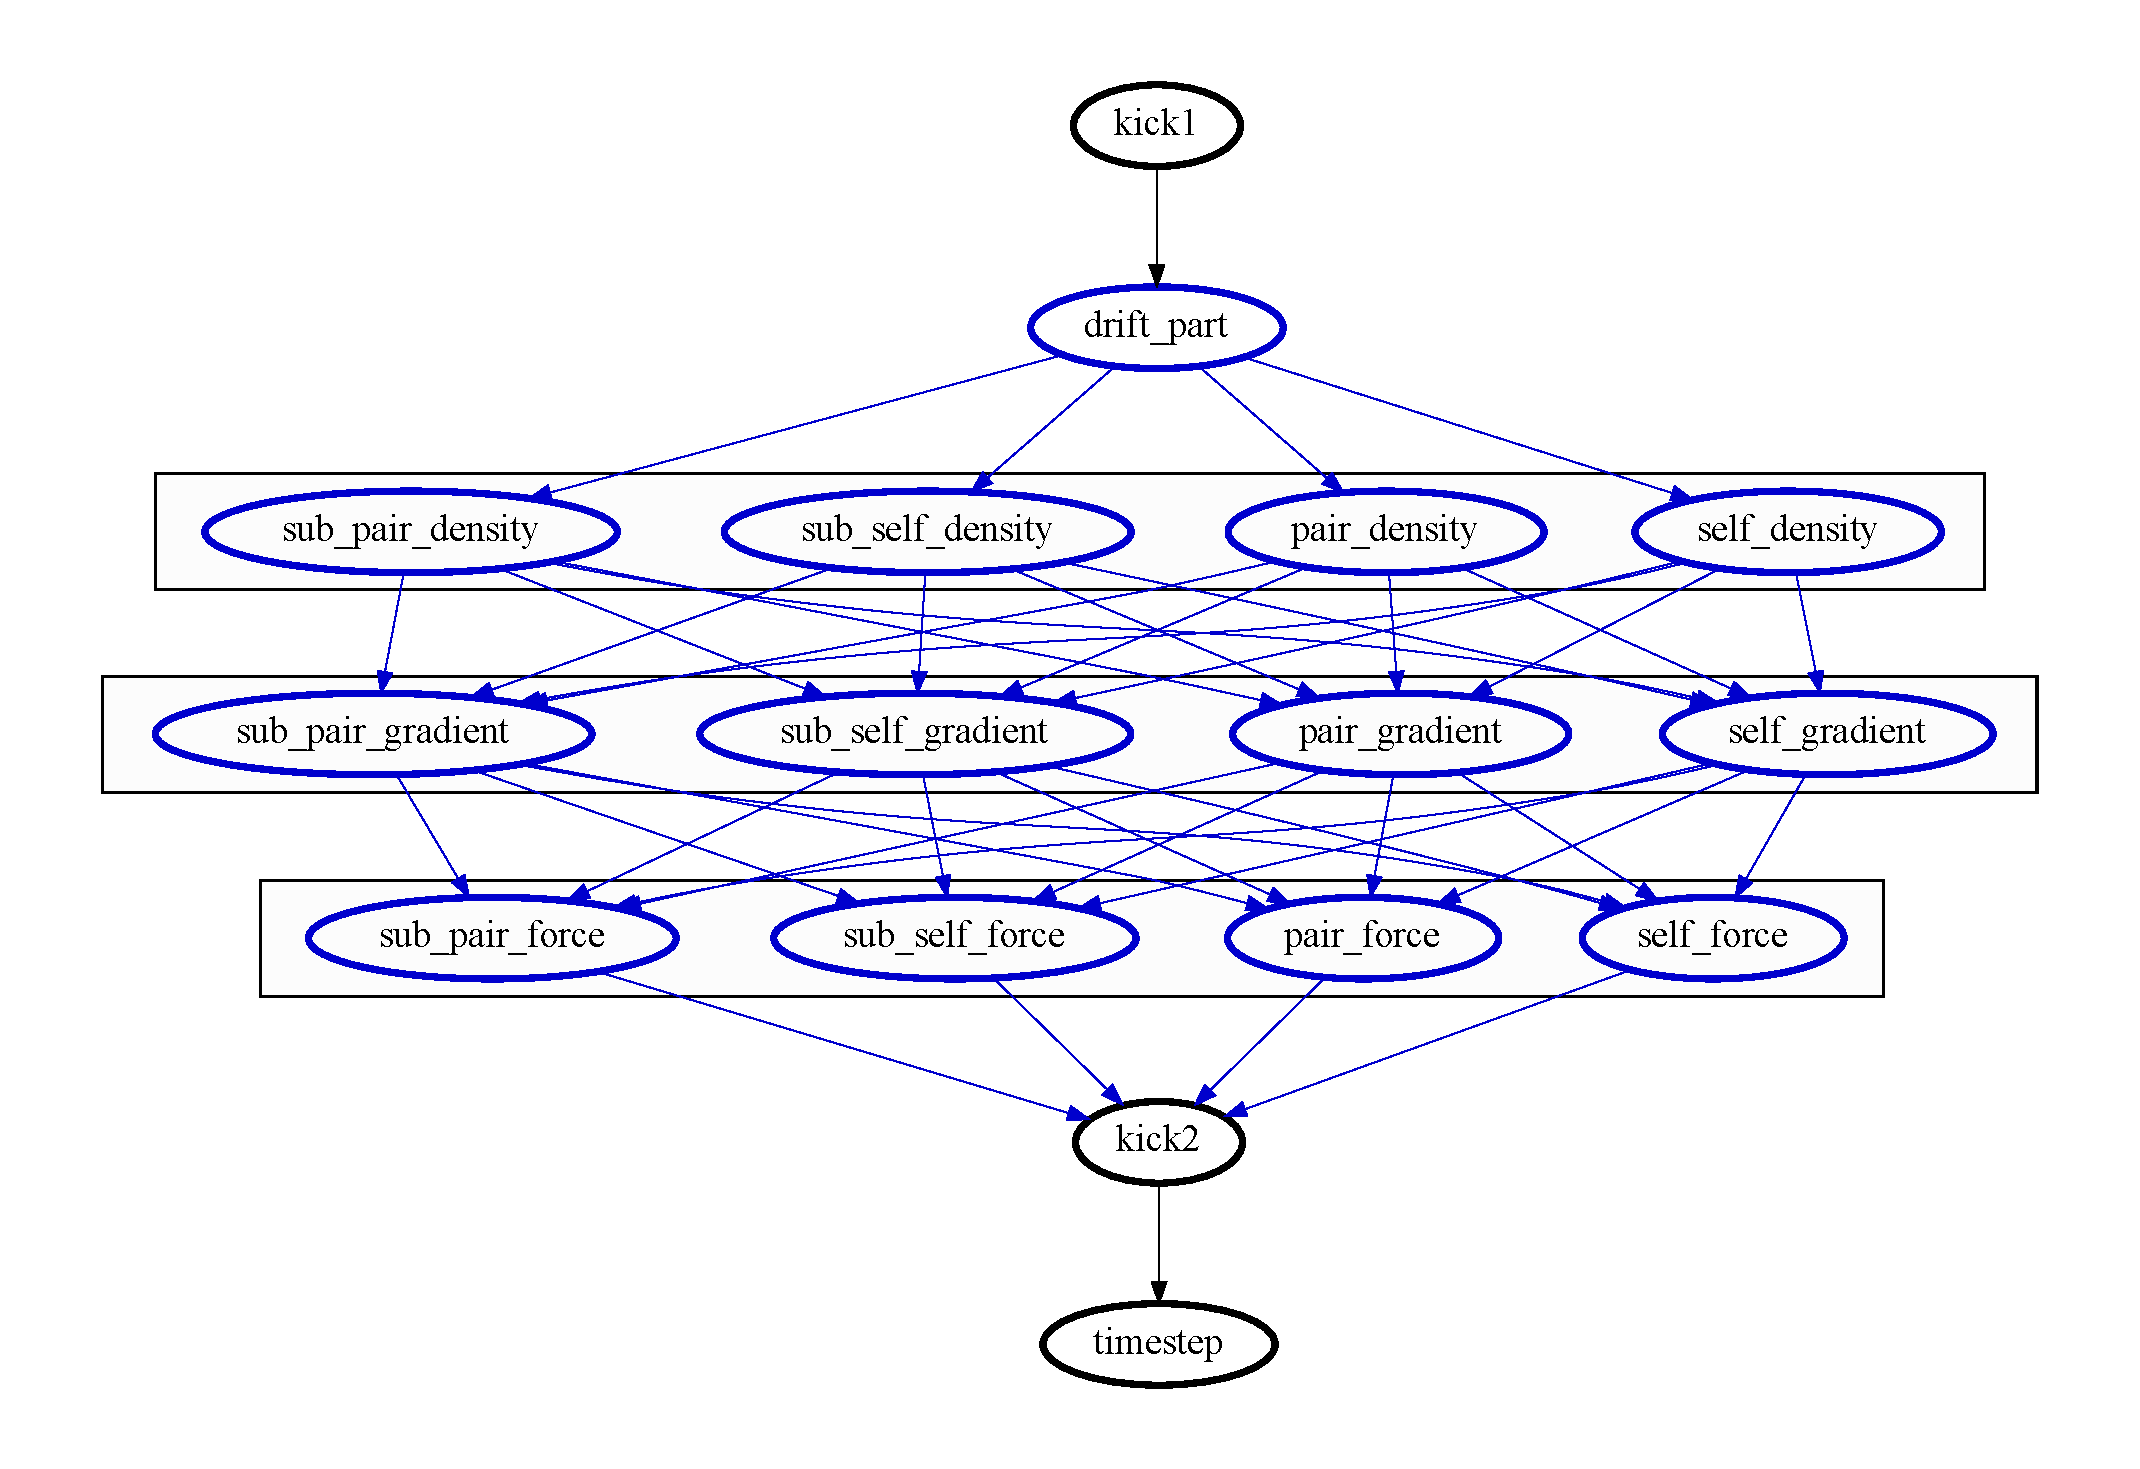
\includegraphics[width=\linewidth]{figures/Meshless/tasks_hydro_zeroth_order.pdf}%
\caption{
A first dependency graph for tasks required for FVPM hydrodynamics with \swift based only on the
required order of operations.
}
\label{fig:dependency-graph-zeroth-order}
\end{figure}


This simplified graph doesn't account for the fact that the required operations which involve
particle interactions can't be modeled exclusively by \lingo{interaction} tasks. Additional work on
individual particles needs to be performed. For example when computing the matrix $\mathcal{B}$
(eq.~\ref{eq:matrix_B}) for the gradients, first the matrix $\mathcal{E}$ (eq.~\ref{eq:matrix_E})
needs to be accumulated as a sum over neighboring particles, and then inverted. The inversion can
only occur \emph{after} $\mathcal{E}$ is accumulated in the gradient interaction tasks, but needs to
happen \emph{before} the flux exchanges in the \lingo{force} tasks. A second example is the fact
that the search for the smoothing length $h$ needs to be performed iteratively. Rather than
repeating all interactions between all neighboring cells, a list of neighbor candidates can be kept
for particles whose smoothing length hasn't converged yet. Only those neighbors can be checked
again. With the lists available after the first interaction task loop, the iteration can be modeled
as a \lingo{plain} task type instead of an \lingo{interaction} type task, which reduces the number
of conflicts in the algorithm. For this reason, new tasks between the density and the gradient, as
well as between the gradient and the force tasks are introduced, called ``\lingo{ghost}'' and
``\lingo{extra\_ghost}'', respectively. The \lingo{ghost} task is called this way because it
technically performs the work of an interaction type task while it isn't one, and hence does the
work in an ``invisible'' manner. These new tasks are shown in
Figure~\ref{fig:dependency-graph-first-order}.

Additionally, two ``\lingo{implicit}'' tasks are added before and after the \lingo{ghost} task,
named ``\lingo{ghost\_in}'' and ``\lingo{ghost\_out}''. \lingo{Implicit} tasks are a third class
of tasks that exists only to collect dependencies, while doing no actual work at all. They are added
an attempt to both reduce the total number of dependencies throughout the entire task graph as well
as to make the code development process easier.



\begin{figure}
\centering
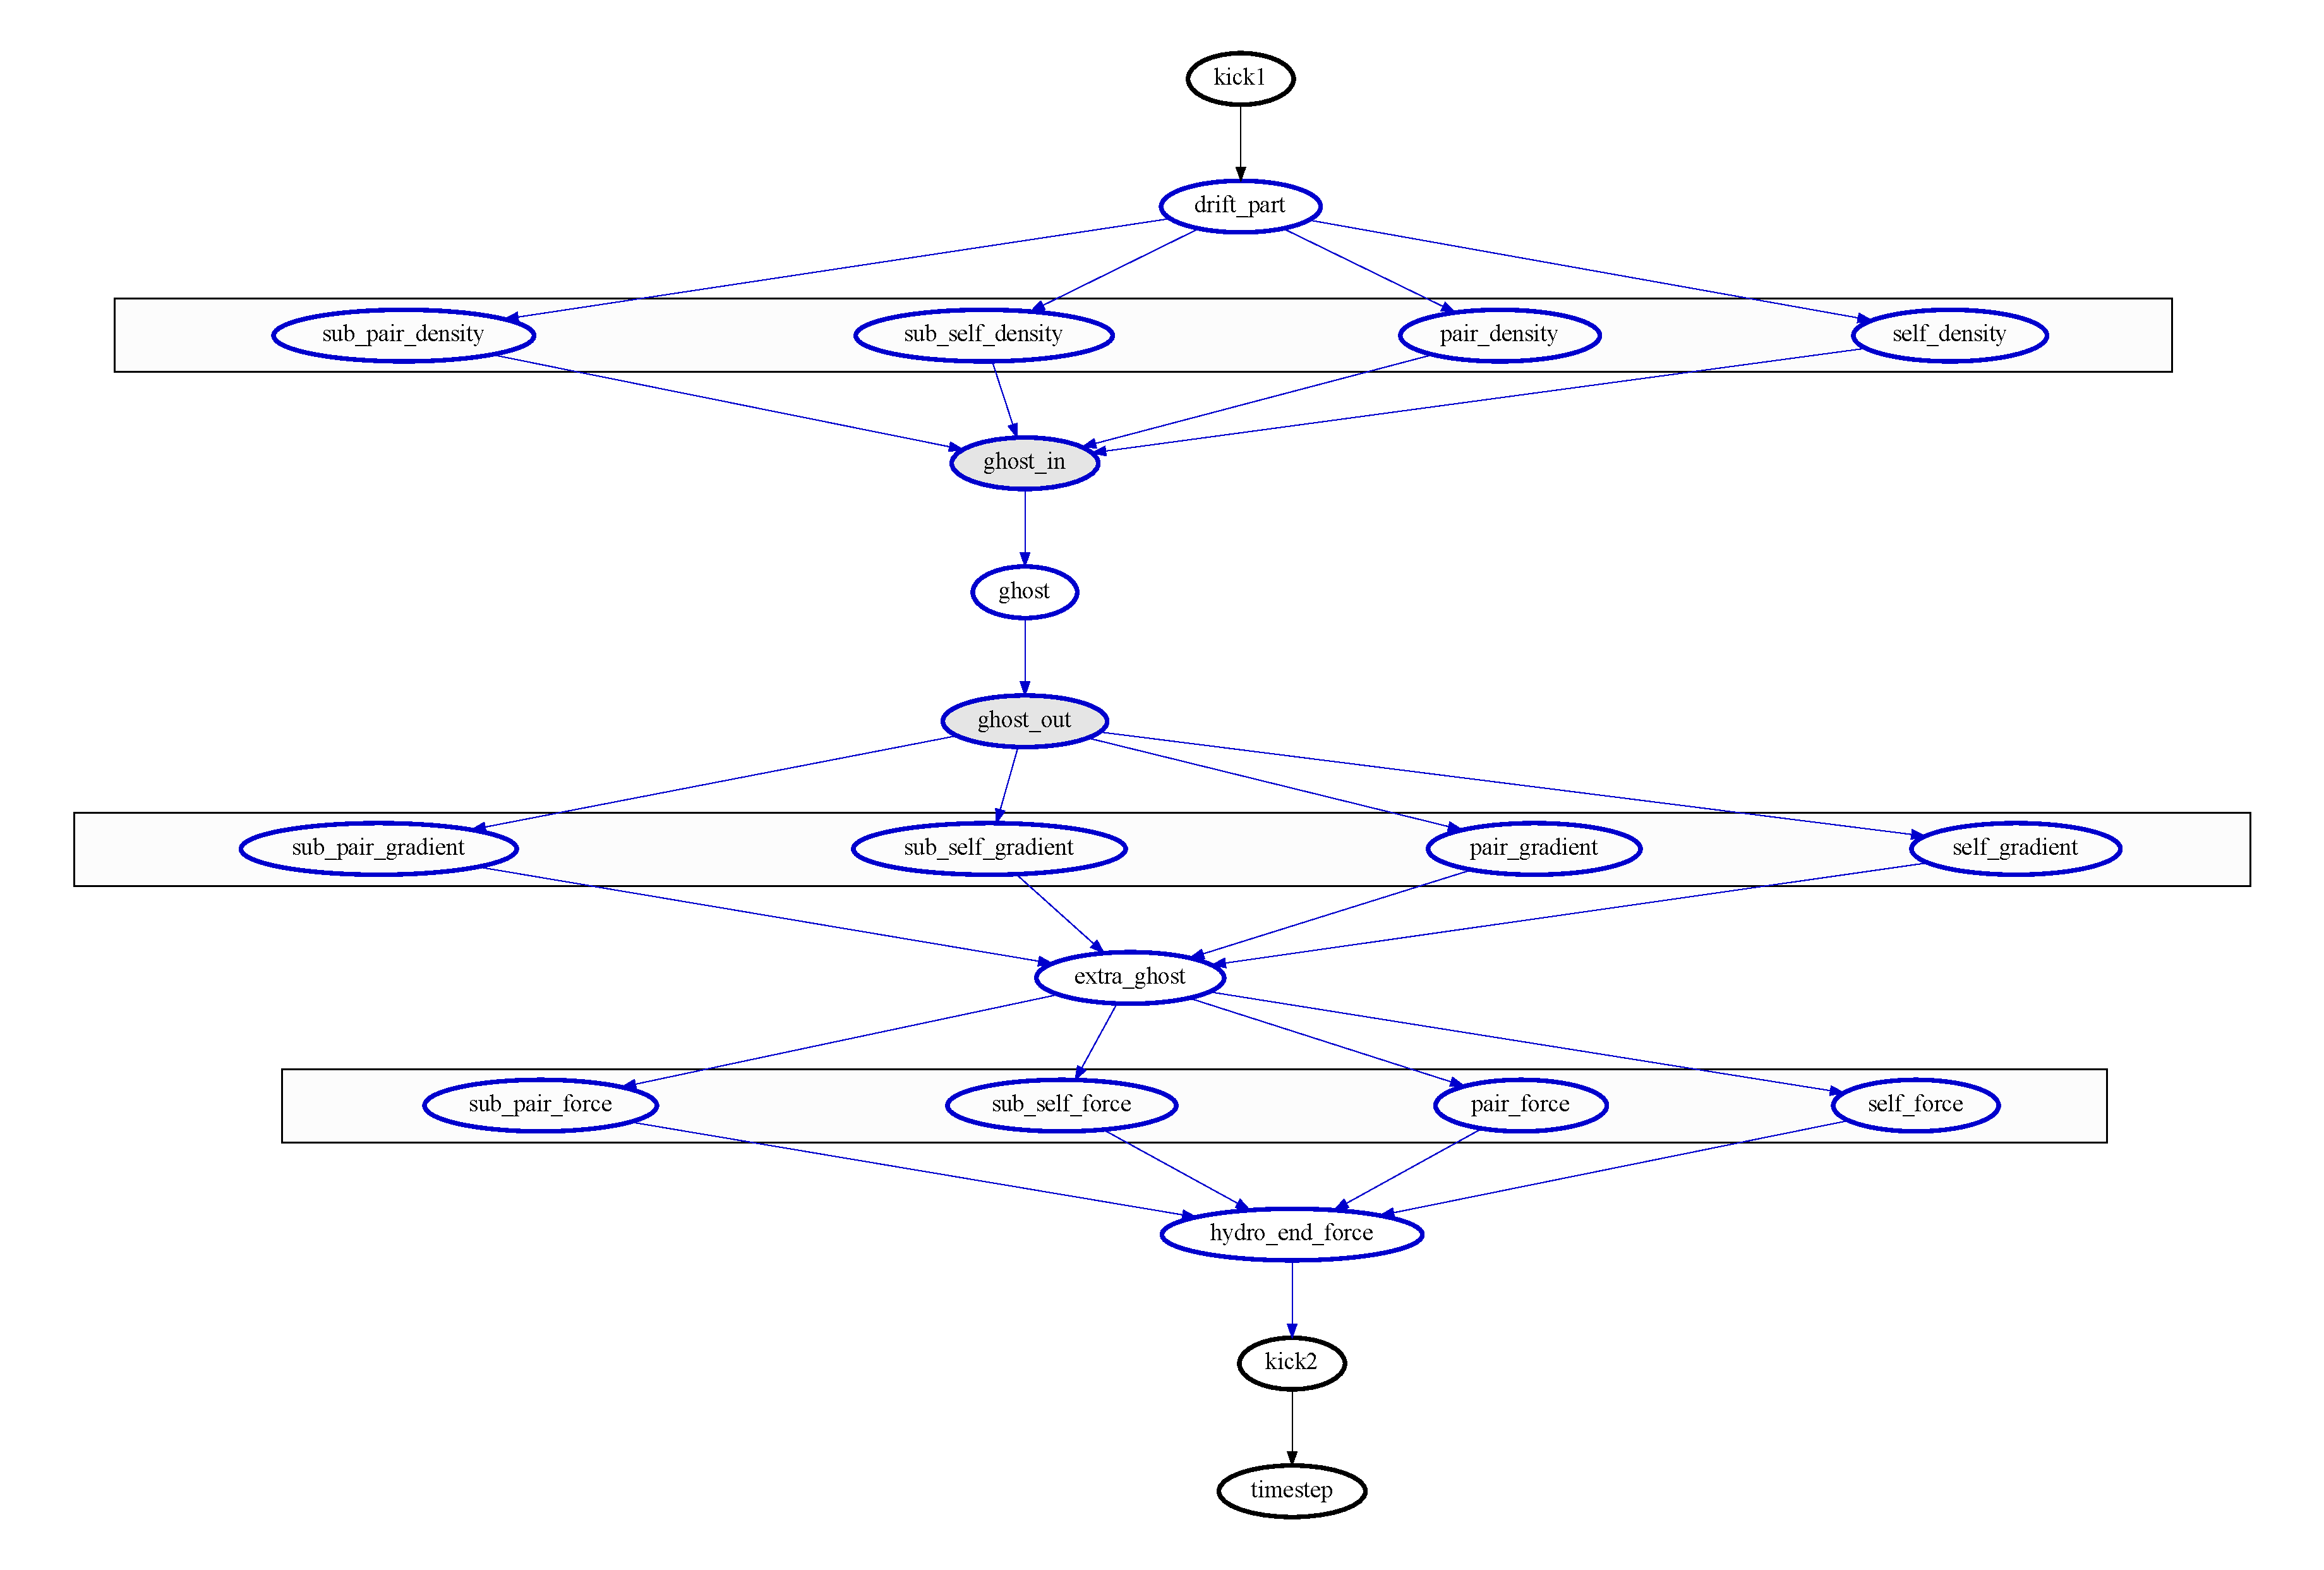
\includegraphics[width=\linewidth]{figures/Meshless/tasks_hydro_first_order.pdf}%
\caption{
A first modification of the dependency graph for tasks required for the hydrodynamics with \swift
with new \lingo{plain} tasks added sandwiched by the \lingo{interaction} type tasks. They are
necessary to complete required computations between the particle interaction operations.
Additionally implicit \lingo{ghost\_in} and \lingo{ghost\_out} tasks have been added (nodes with
gray background). They perform no actual work themselves, and exist only to collect dependencies and
make the development process easier.
}
\label{fig:dependency-graph-first-order}
\end{figure}




%--------------------------------------------------------------------------
\subsection{Optimizing \lingo{Pair}-Type Interactions: Sorting Cells}
%--------------------------------------------------------------------------

The interactions between particles constitute a major part of the total workload each time step. For
the finite volume particle methods, we require three separate loops over neighboring particles.
Given this prevalence of the particle interactions, it is sensible to invest effort towards
optimizing the way particle interactions are performed. A good starting point is to limit the total
number of particles checked for possibly being neighbors even more than is already done by
constructing cells in a manner such that all neighbor particles must be situated within adjacent
cells. To this end, particles inside each cell are sorted along each of the 13 lines connecting a
cell center with an adjacent cell center. Any cell will have 26 adjacent cells of equal size, with
each of these 26 neighboring cells having a diagonally opposed counterpart. So it suffices to sort
the particles only along half of the 26 axes, and use the reverse order of the sorted list for the
diagonally opposed neighbor cells. The lists of sorted particles are then used in pair and sub-pair
type tasks as a means of reducing the number of viable possible neighbor particles during an
interaction loop by traversing the sorted lists rather than traversing all particles in the
neighboring cell. More precisely, instead of checking whether each particle in the first cell is
within range of each particle of the second cell, both cells' particles are traversed in the sorted
order along the axis that connects the cells' centers. The distance of the particles on the sorting
axis gives a lower limit on the actual distance between the two particles, since their positions
have been projected along the axis for the sorting. This way a significant amount of unnecessary
checks can be avoided. To facilitate the sorting, ``\lingo{sort}'' tasks must be added, which is
shown in Figure~\ref{fig:dependency-graph-second-order}. The sorting must take place after the
drifts, during which the particle positions are being modified, and before the \lingo{pair} and
\lingo{sub-pair} type tasks. Note that the \lingo{self} type tasks, which only interact particles
within a cell with other particles inside the same cell, do not require the cell itself to be
sorted, and hence have no dependency on the \lingo{sort} task. The \lingo{sub-self} tasks however
recursively interact particles of their child cells with each other, which again needs the particles
in the child cells to be sorted.


\begin{figure}
\centering
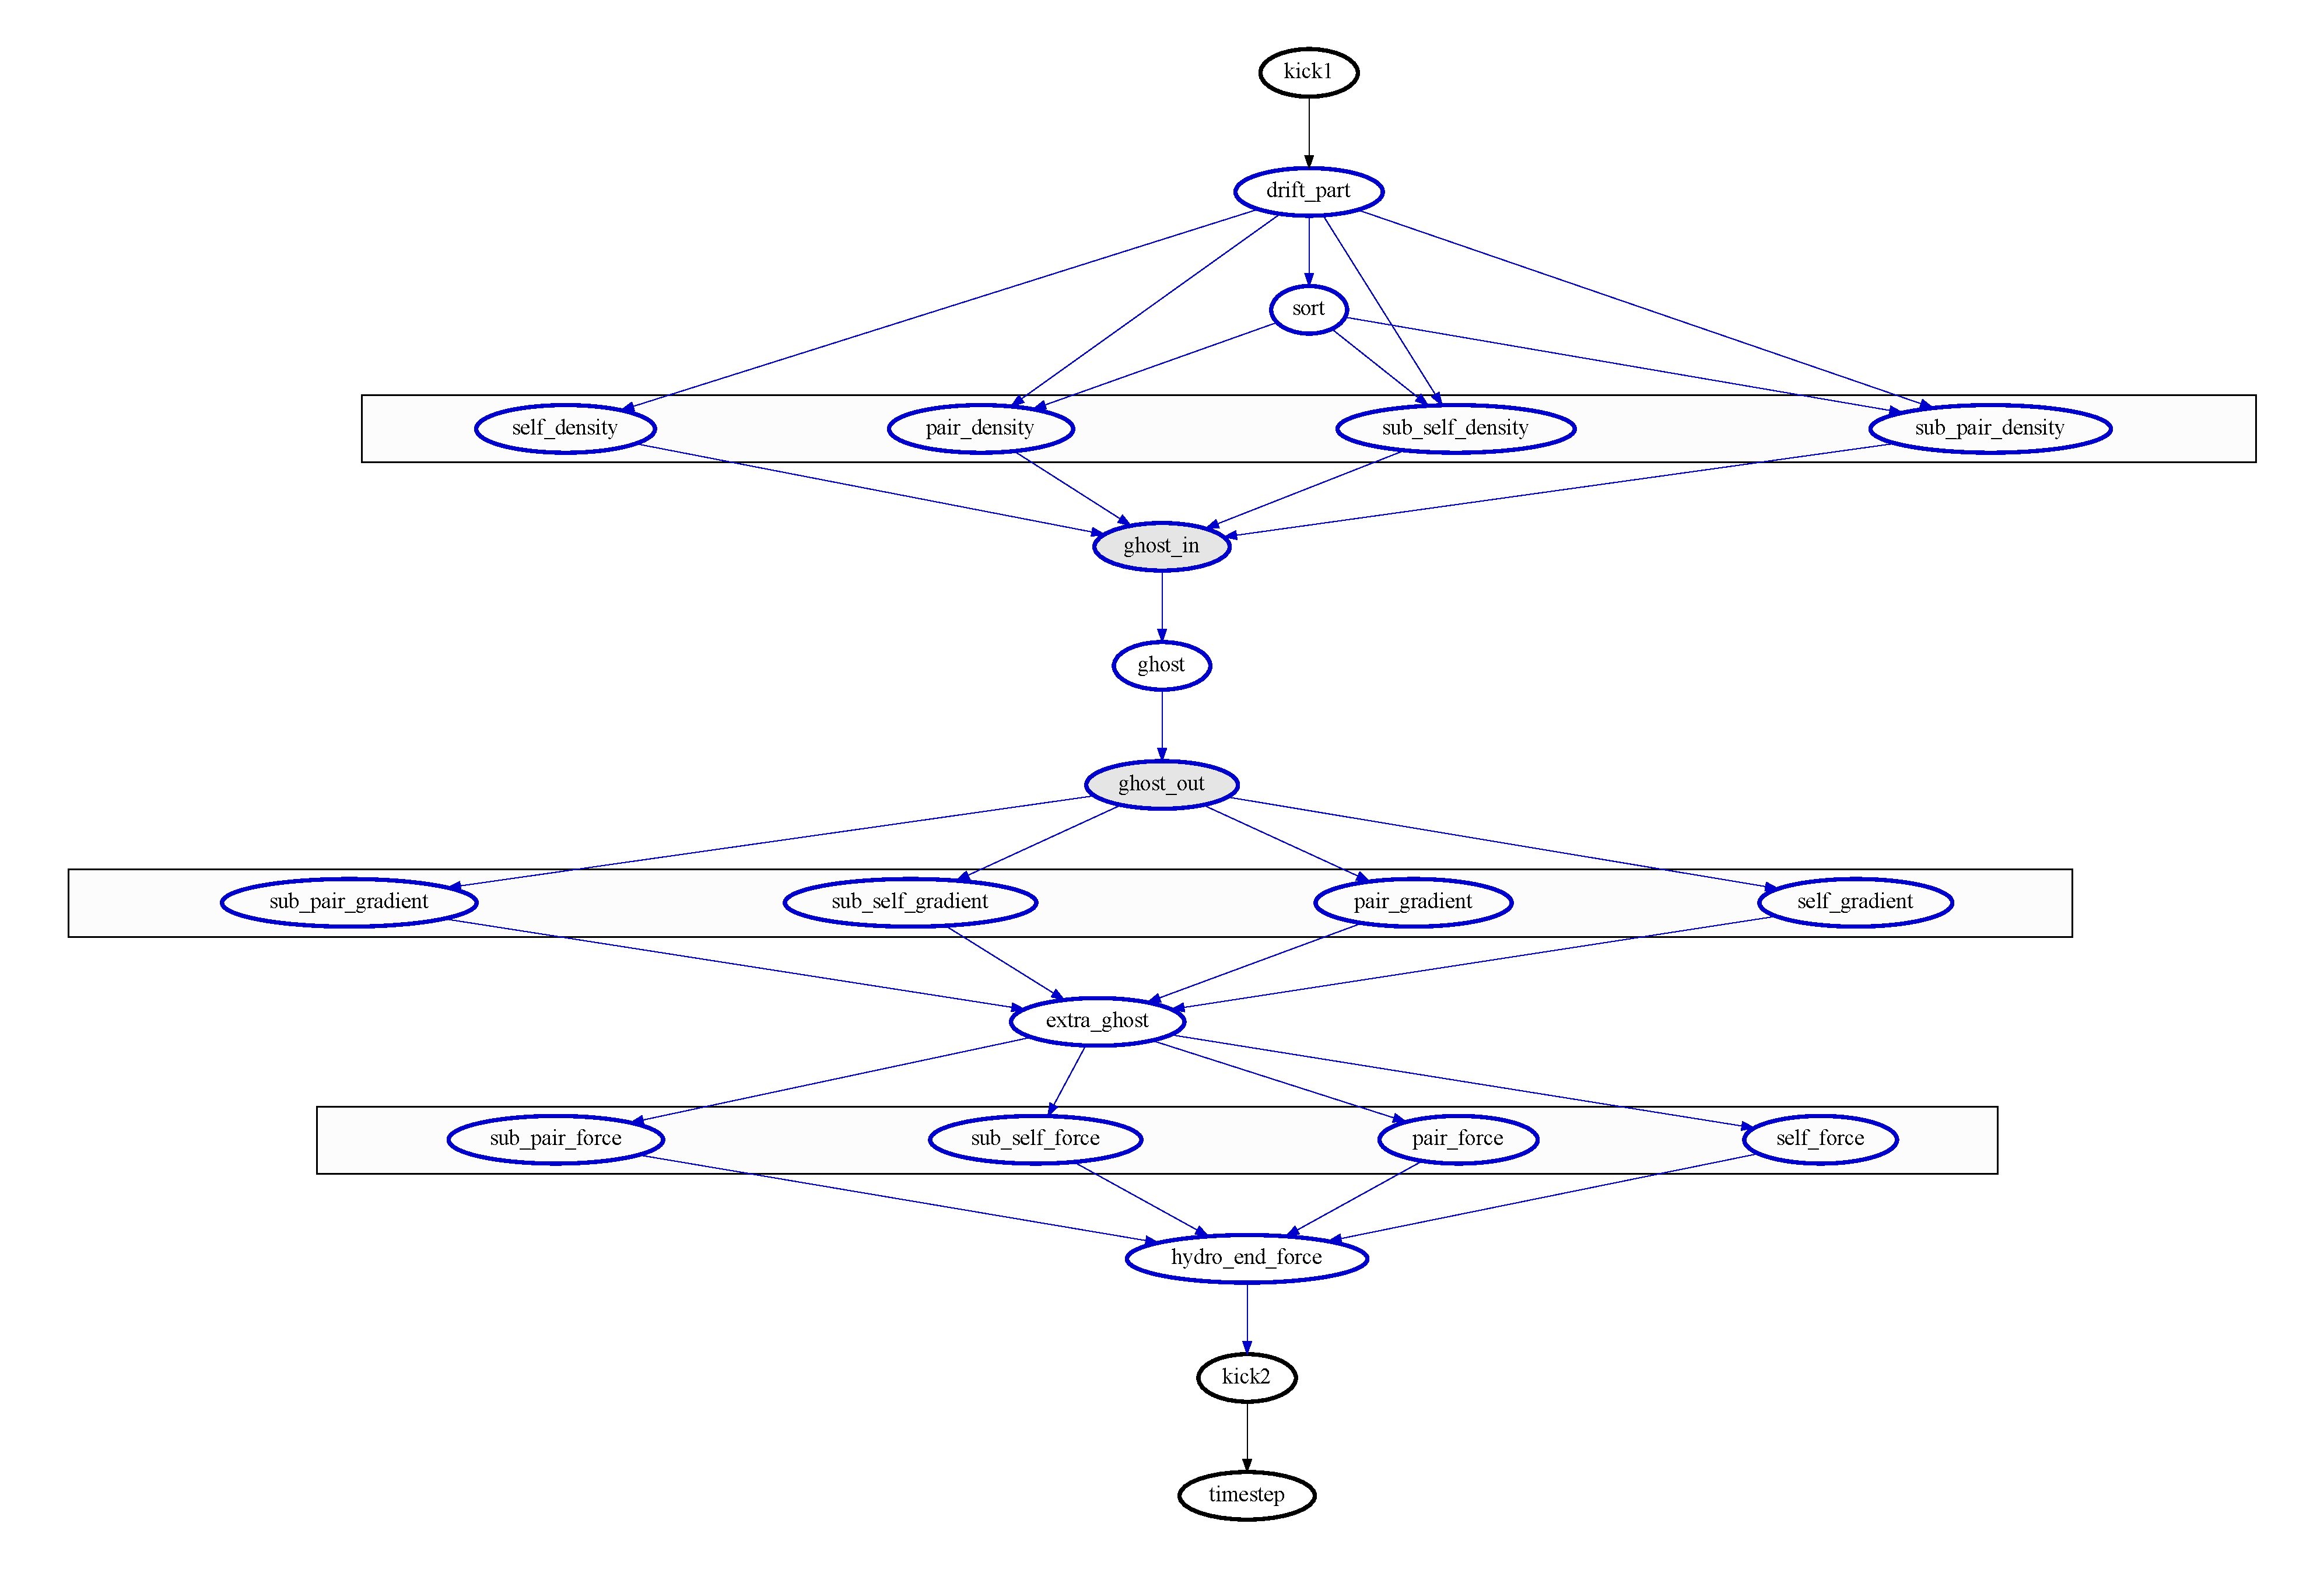
\includegraphics[width=\linewidth]{figures/Meshless/tasks_hydro_second_order.pdf}%
\caption{
The second modification of the dependency graph for tasks required for the hydrodynamics with
\swift, with the \lingo{sort} task and its dependencies added.
}
\label{fig:dependency-graph-second-order}
\end{figure}








%--------------------------------------------------------------------------
\subsection{Adapting to Individual Time Step Sizes of Particles}
%--------------------------------------------------------------------------


The next required modification is necessary to facilitate the individual time steps for particles
(see Section~\ref{chap:individual-timesteps}). Consider a case where some
particle $i$ has a time step of size $\Delta t$ with a neighboring particle $j$ which has a time
step of size $2 \Delta t$. Allowing the particles to have individual time steps would mean that
while particle $i$ does two time step integrations following its own time step size $\Delta t$,
particle $j$ does only one. During the second update of particle $i$, while particle $j$ is
skipped, particle $i$ needs to go through its entire required order of operations, which includes
the neighbor search to determine the smoothing length $h$. However $h$ depends on the neighboring
particle positions, so for $h$ to be accurate, all neighboring particle positions must be correct,
i.e. drifted to the correct time. This means that particle $j$ would need to be drifted to a time at
 which it is not being integrated itself because particle $i$ requires it (see
Figure~\ref{fig:individual-time-steps-drifts}). Luckily drifting the particle positions is a linear
operation, which can be exploited. Let $K(\Delta t)$ denote the kick operation for a particle, and
$D(\Delta t)$ denote the drift operation. For particle $j$, which has a time step size of $2 \Delta
t$, a kick-drift-kick time integration can then be written as
\begin{align}
    K(\Delta t) \circ D(2 \Delta t) \circ K(\Delta t)
\end{align}

However, since the drift operation is linear, we can just as well do


\begin{align}
    K(\Delta t) \circ D( \Delta t ) \circ D(\Delta t) \circ K(\Delta t) \\
    = K(\Delta t) \circ D( \Delta t / n ) \circ \hdots \circ D(\Delta t / n) \circ K(\Delta t)
\end{align}

So we can concatenate any number $n$ of drift operations on a particle between the two kick
operators. This means that as long as the first kick operation on particle $j$ has been performed
already, we can keep drifting the particle $j$ even in time steps where it is skipped so the
neighboring active particle $i$ has access to the correct positions of its neighbor. To this end,
we perform the following modifications: When a simulation starts, the first kick operation is
performed on all particles. This way, we can begin each subsequent simulation time step with the
drift operation. If a particle is being skipped in the current time step due to its larger
individual time step size, then it will be in the correct state to be drifted to the current time.
These drifts can be repeated an arbitrary number of times until the time is reached where the
particle undergoes a full hydrodynamics step itself. The first kick operation is then moved in the
task dependency graph from being at the root of the dependency graph (like in
Figure~\ref{fig:dependency-graph-second-order}) to the end (see
Figure~\ref{fig:dependency-graph-nompi}), after the new time step size for a
particle has been computed in the timestep tasks. Once the particle has done its first kick
operation, it is once again in the correct state to be drifted any required number of times until
its own next time step begins. Figure~\ref{fig:individual-time-steps-drifts} shows how the kick and
drift operations are performed with three interacting particles with different time step sizes.


\begin{figure}
 \centering
 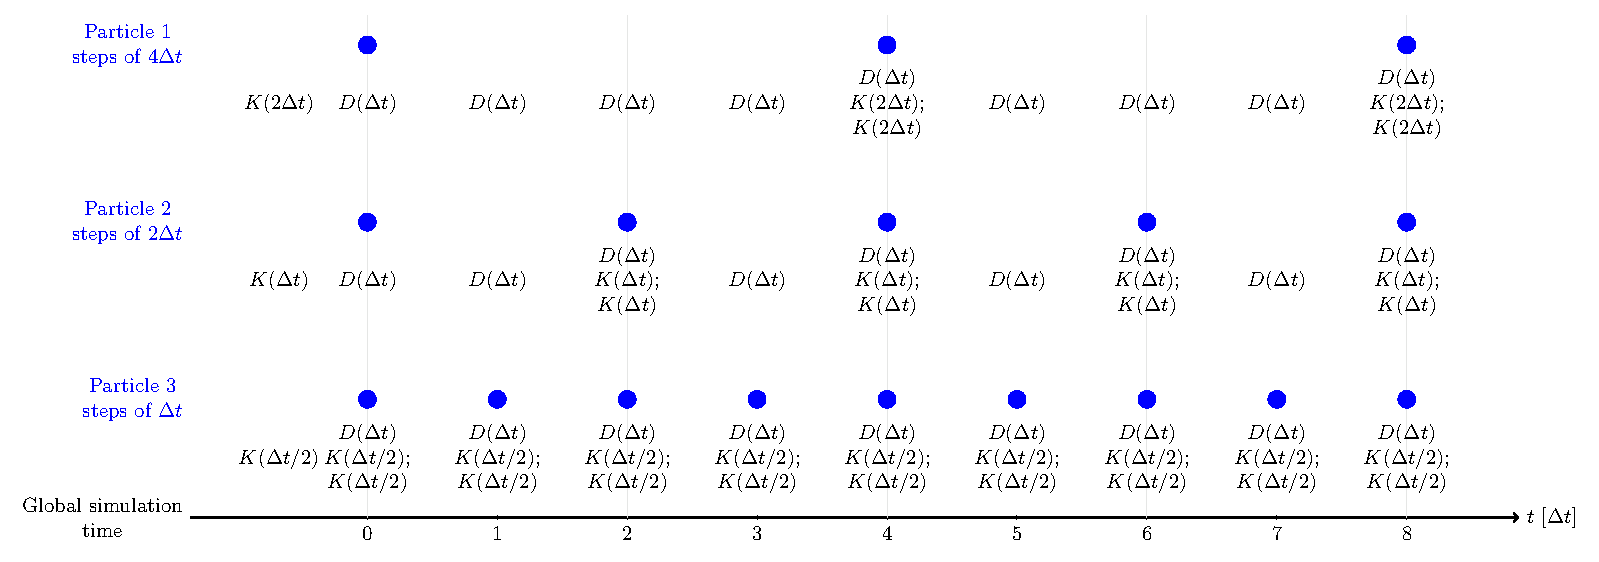
\includegraphics[width=\textwidth]{figures/Meshless/individual_timestepping_operators.pdf}%
 \caption{
Illustration of how the kick and drift operations are performed for particles with individual time
step sizes. A full time integration for a particle with time step size $\Delta t$ is given by
$K(\Delta t / 2) \circ D(\Delta t) \circ K(\Delta t/2)$, where $K$ denotes a kick operator, and $D$
denotes a drift operator. Three particles with time step sizes $\Delta t$, $2 \Delta t$, and $4
\Delta t$, respectively, are depicted. The blue dots represent the points in the simulation time
(shown on the x-axis) at which the respective particles undergo a full hydrodynamics integration
update, i.e. complete the kick-drift-kick integration. Between the full updates, particles with
higher time step sizes compared to their neighbors are drifted to the current simulation time so
their neighbors, which finish their integration step in this simulation step, have access to the
correct particle positions. In order for all particles to be in the correct state to be drifted any
number of times, the first kick operator is applied to all particles before the first simulation
step. At the end of a simulation step, the particles aren't left in the state where the integration
step finishes, i.e. after the second kick operator has been applied, but are kicked again with their
new time step size. This way, they can again be drifted any number of times until the simulation
reaches the step where the particle completes its own time integration step.
 }
 \label{fig:individual-time-steps-drifts}
\end{figure}






%----------------------------------------------------------
\subsection{Facilitating Task Activation}
%----------------------------------------------------------

There is one more additional task required before we can turn our attention towards how to deal
with distributed memory architectures. This task is related to the \emph{task activation}. The
tasks themselves as structures that contain information what work is to be performed on a cell are
created when the cells themselves are created. Before a simulation step is executed, tasks are
activated depending on whether the work they represent needs to be performed in the following
simulation step. This is not always the case: For example, while one cell may contain particles
that finish their time step in this simulation step, there may be cells somewhere else in the
simulation which contain no particles that require an update in this simulation step. A cell which
contains particles that need to be updated in the current simulation step is called
``\lingo{active}'', otherwise ``\lingo{inactive}''. Only tasks which perform work on an
\lingo{active} cell are also activated, i.e. passed to the scheduler for subsequent execution.

In order to facilitate this task activation, cells need to store the information whether they
are \lingo{active} at the current simulation time. For split cells, this information needs to be
available recursively for their child cells as well. This information is gathered and stored for
each cell during the \lingo{timestep} tasks. \lingo{Timestep} tasks are the ones where the new time
steps for particles that reside in that cell are computed after the integration step of the
particles is complete. Similarly, the information also needs to be available to the parent cells of
the cells to which tasks are attached to. Recall that tasks are attached to the \lingo{super level}
in the tree, which may or may not be the \lingo{top level}. This work is performed by the
``\lingo{collect}'' task, whose only purpose is to recursively pass on the activity information
from the \lingo{super level} to the \lingo{top level}. The \lingo{top level} cells require the
activity information because the task activation is performed recursively starting at the
\lingo{top level}. When other physics (or more precisely other particle types than particles
representing the fluid) like gravity are included in the simulation, the corresponding tasks can
have a \lingo{super level} which is different from the \lingo{super level} of the hydrodynamics
tasks. To ensure that the task activation process is performed correctly, it needs to begin at the
root of the cell tree, which is the \lingo{top level}.



\begin{figure}
 \centering
 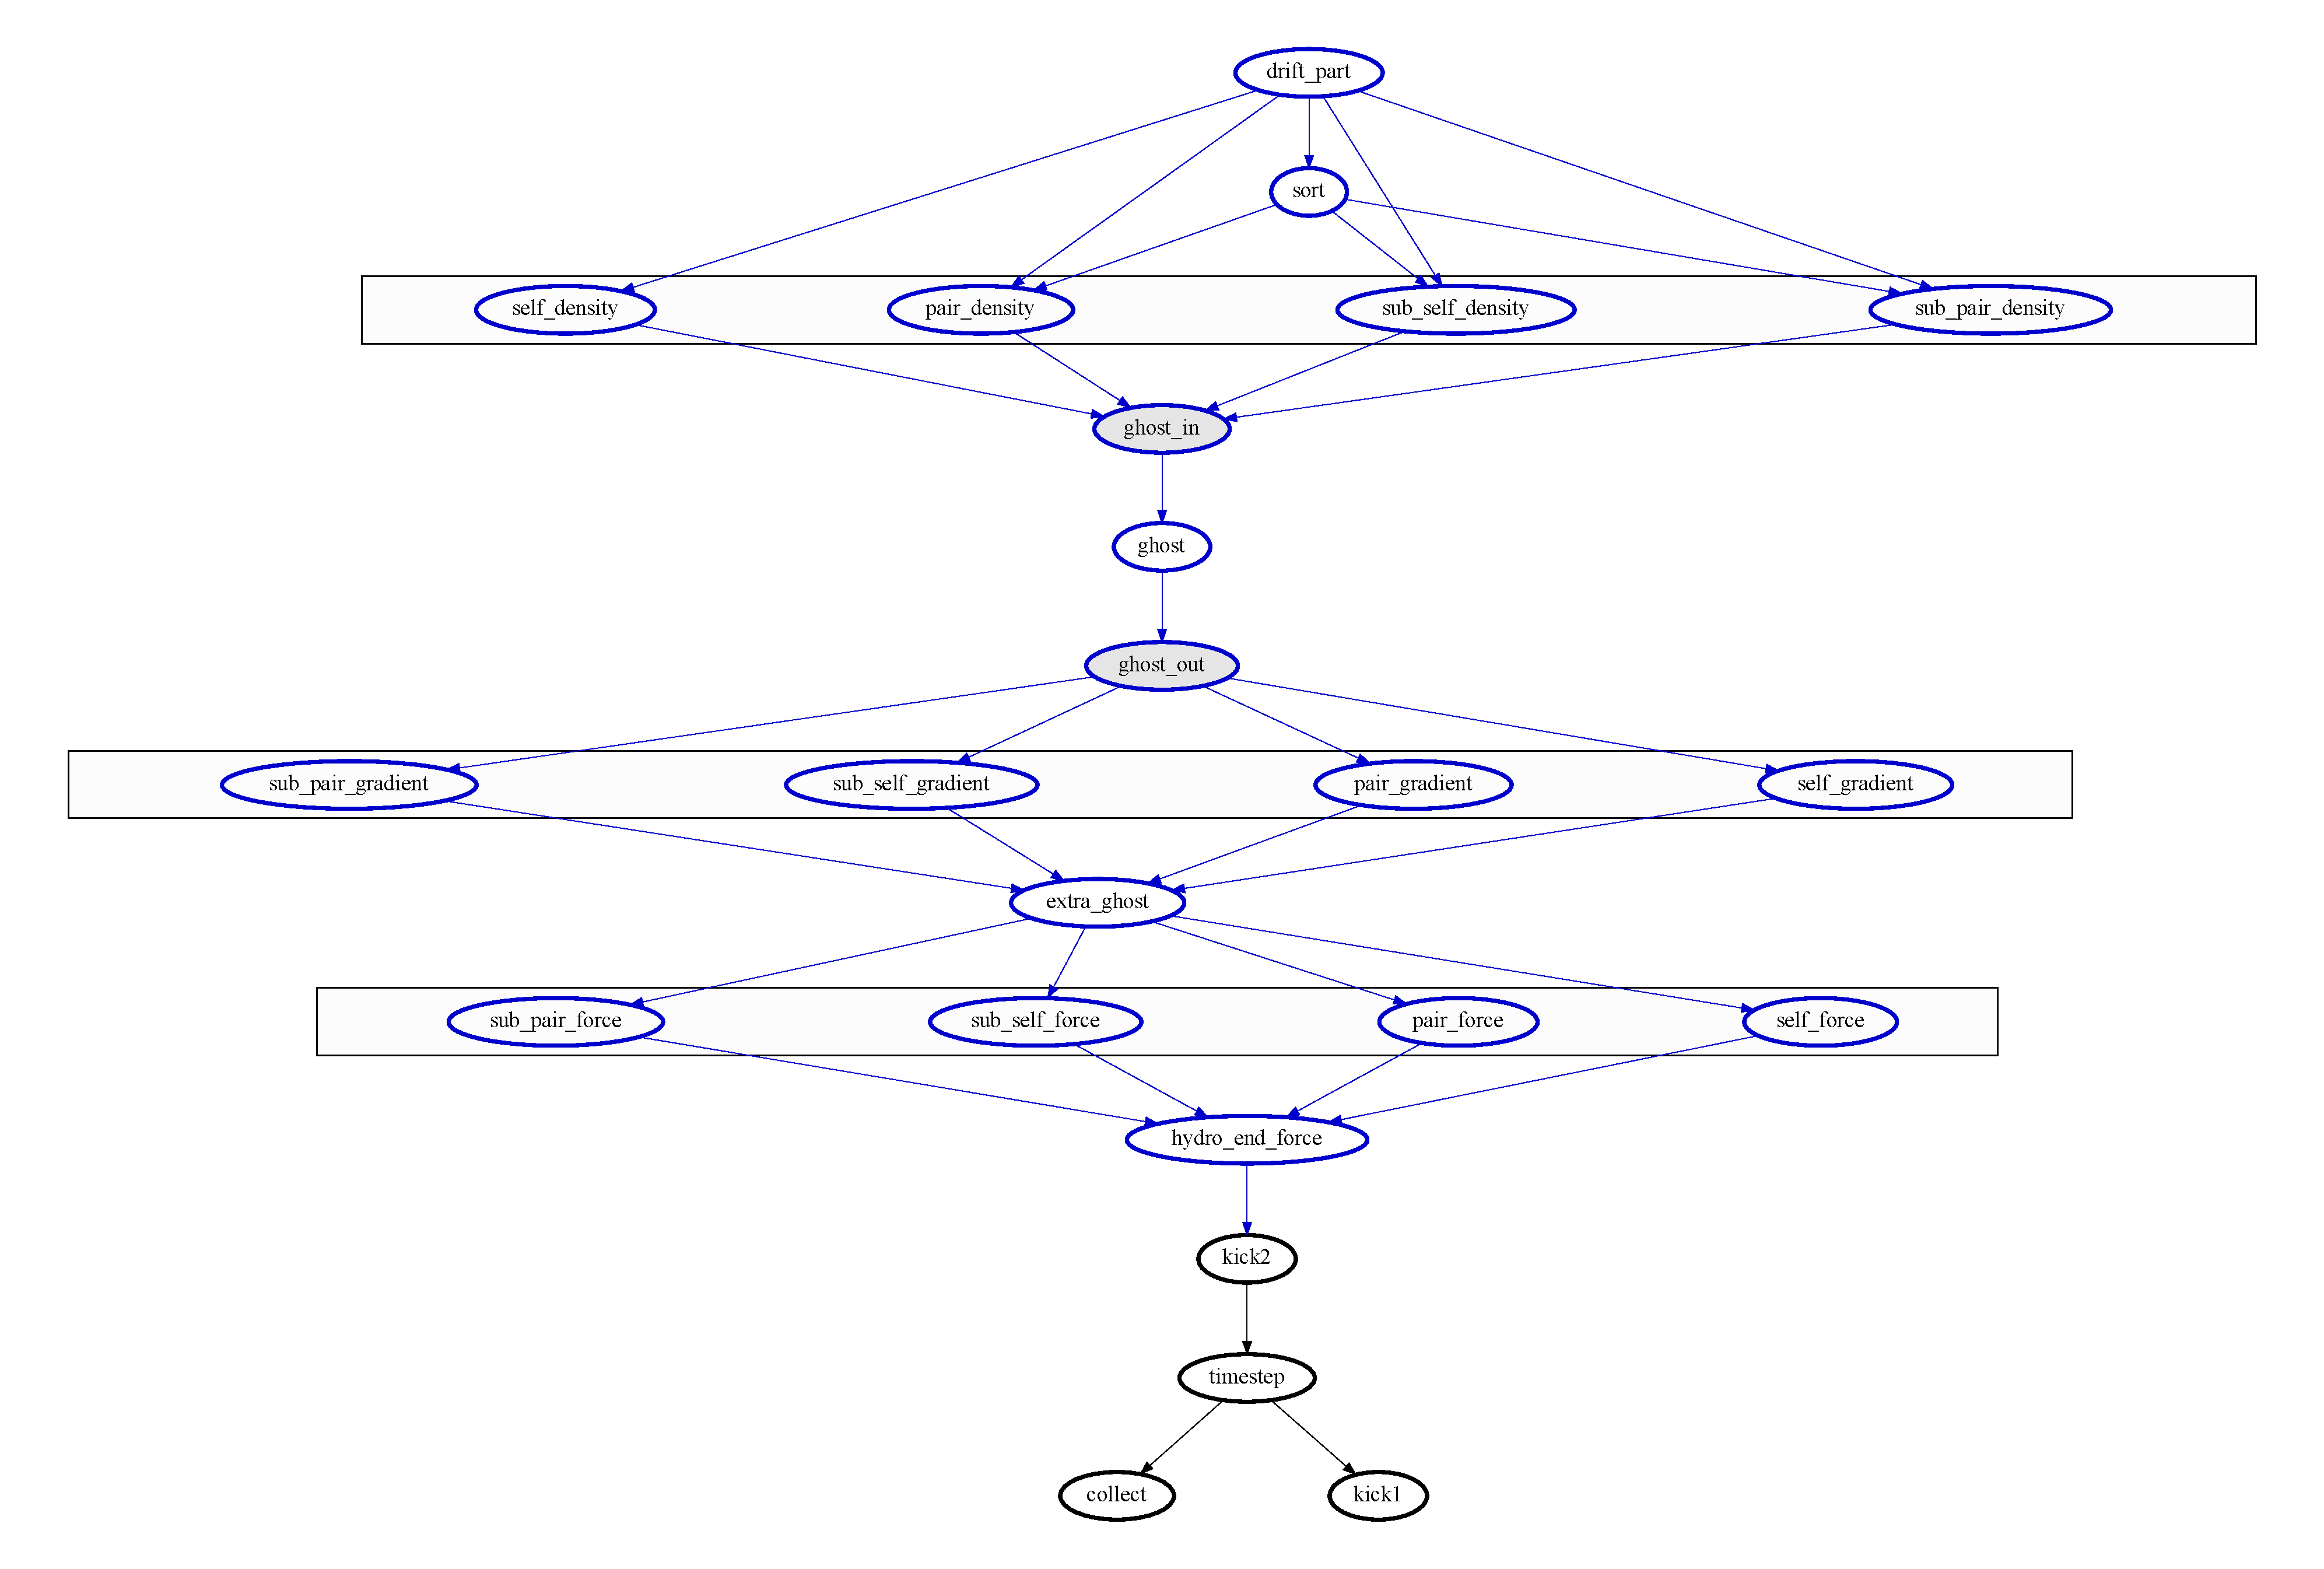
\includegraphics[width=\textwidth]{figures/Meshless/tasks_hydro_nompi.pdf}%
 \caption{
The dependency graph for tasks required for the hydrodynamics with \swift for shared memory
architectures. The \lingo{kick1} task has been moved to the bottom of the dependency graph, and the
\lingo{collect} task has been added.
}
 \label{fig:dependency-graph-nompi}
\end{figure}





%------------------------------------------------------------------------------
\subsection{Distributed Memory Parallelism: Domain Decomposition and MPI}
%------------------------------------------------------------------------------


This concludes the construction of the dependency graph for finite volume particle hydrodynamics
with \swift on shared memory architectures, where all threads have access to all data at all times.
Modern high performance computing software however needs to go beyond shared memory architectures to
be able to solve sizable problems: There are limits to how many CPUs can have access to the same
blocks of memory before the architecture becomes too expensive, too inefficient, or even impossible
to create. In order to be able to increase the computing power beyond the capabilities of one node,
or shared memory region, these nodes can instead be connected in a network and form a distributed
memory architecture. However, the CPUs between different nodes (individual regions of shared
memory) have no access to each others respective memory, and necessary data needs to be communicated
between the nodes explicitly. The industry standard for such communications is the ``Message
Passing Interface'' MPI, which defines a standard for the communications and has several available
implementations. In MPI terminology, each separated memory region with associated CPUs is called a
``\lingo{rank}''. While the main benefit of MPI is the possibility to pass messages between
different nodes, MPI is perfectly capable of running several \lingo{ranks} on a single node as
well. However, each \lingo{rank} still only has access to its own data, even when being executed on
the same node, where in principle the memory can be shared between CPUs.






%------------------------------------------
\subsubsection{Domain Decomposition}
%------------------------------------------

At its core, the strategy to run simulations on distributed memory architectures is to split the
entire problem into separate regions and assign a region to each MPI rank. This process is called
``domain decomposition''. To illustrate this process, suppose that the simulation you'd like to run
consists of a square. A very simple domain decomposition would be to split the square in half and
give each half of the total square to an individual MPI \lingo{rank} to work with, as is shown in
Figure~\ref{fig:domain-decomposition}. Communications become necessary when a \lingo{rank} requires
data which is stored on a different \lingo{rank}: For example, consider a particle-particle
interaction loop along the edge of a the halves of the square. Particle data along the edges of each
half needs to be sent to the other \lingo{rank}, and vice versa. While the communications are extra
work that needs to be performed, and hence constitute an overhead, a significant advantage is that
through MPI the total amount of memory available for a problem increases.\footnote{
Additionally, since MPI is capable of running multiple \lingo{ranks} on shared memory architectures
just as if it were a distributed memory architecture, it can be used as a method to parallelize
serial software on shared memory architectures as well. An MPI only parallelization for shared
memory architectures will almost certainly not be as efficient as a dedicated shared memory
parallelization method due to the overheads it involves. However, it would still constitute an
improvement over strictly serial code.}
For example if we use two MPI \lingo{ranks}, like in Figure~\ref{fig:domain-decomposition}, and
assign one \lingo{rank} per computing node, then we can use the entire memory available on two
nodes, rather then one, and fill the memory with twice\footnote{Not accounting for additional
overheads that arise due to the addition
of MPI and domain decomposition.}  as many particles than before.

The separation of the work into individual tasks required for the task-based parallelism in
\swift allows us to make more sophisticated choices for the domain decomposition than a simple
geometrical partition of the volume. The computational load for each MPI \lingo{rank} can be
modeled much more accurately using tasks rather than basing the decomposition on equal volumes or
particle counts. This allows for better load balancing between each MPI \lingo{rank}, and hence
reduces idle times of entire \lingo{ranks} which are waiting for other \lingo{ranks} to finish
their respective work. Furthermore, the number of communications can be drastically reduced by
splitting the domain along regions with large time step sizes of particles. For example, it is much
more preferable to split the domain in regions largely void of particles rather than splitting the
center of a galaxy, where particles tend to have very short time steps. Large time step sizes means
that fewer time integrations for these particles are necessary, and hence fewer total communications
and associated overheads are required. So using the data available through the existence of tasks
can both optimize the load balancing as well as minimize the number of necessary communications.
This is achieved by modeling the domain, the work associated with it, and the communications as a
graph, and making use of the graph partition library \codename{Metis}
\citep{karypisFastHighQuality1998} to optimize the domain decomposition.

\begin{figure}
 \centering
 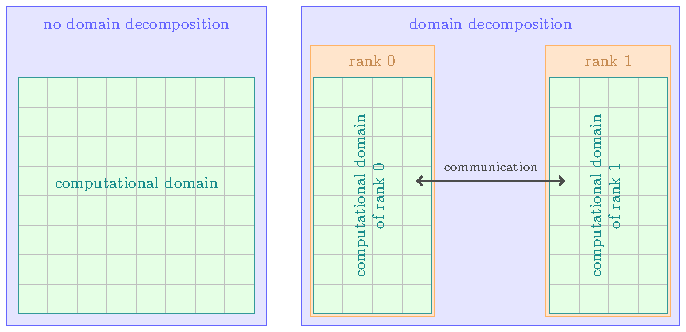
\includegraphics{figures/Meshless/domain_decomposition.pdf}%
 \caption{
Schematic illustration of the domain decomposition strategy for distributed memory architectures:
The initial total volume is split between the two \lingo{ranks} in this example. Splitting the
domain requires communications of necessary data between the \lingo{ranks}. However, thanks to the
possibility to solve the problem on separate \lingo{ranks}, a much bigger problem can be solved. In
this example we can use the total memory of two computing nodes instead of only one.
 }
 \label{fig:domain-decomposition}
\end{figure}







%---------------------------------------------------------------
\subsubsection{MPI Communications}
%---------------------------------------------------------------


\begin{figure}
 \centering
 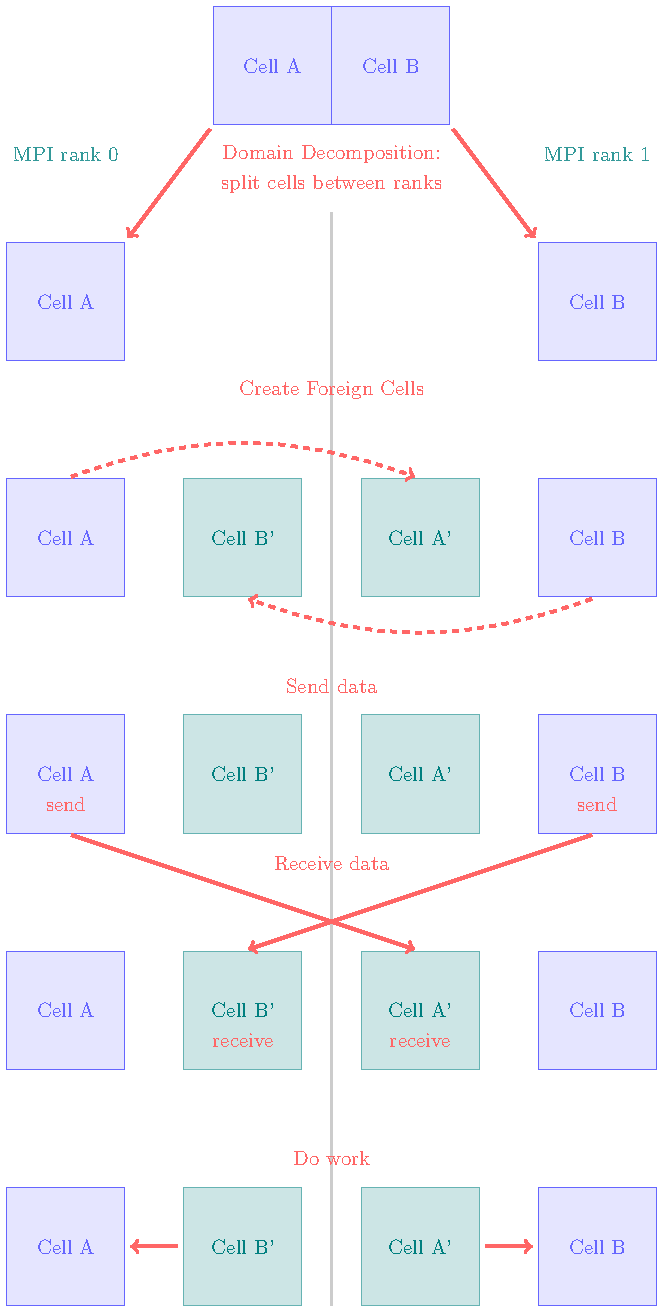
\includegraphics[height=.8\textheight]{figures/Meshless/mpi_comm.pdf}
 \caption{
Sketch on how the MPI communications with a decomposed domain work. Two cells, $A$ and $B$, first
get assigned to two different MPI \lingo{ranks} during the domain decomposition, and a
\lingo{foreign} counterpart cell $A'$ and $B'$ is created on the other \lingo{rank}, respectively.
A
communication then consists of the following order of operations: First the \lingo{real} cells $A$
and $B$ send their data to the foreign counterparts $A'$ and $B'$, respectively. The
\lingo{foreign}
cells $A'$ and $B'$ receive data when the corresponding \lingo{receive} tasks are executed. Finally
the work can proceed, and the \lingo{real} cells $A$ and $B$ can updated correctly. Note that
\lingo{foreign} cells are never updated on foreign \lingo{ranks}, only \lingo{real} cells are
updated. \lingo{Foreign} cells' only purpose is to make the necessary data available for other
\lingo{real} cells on their respective \lingo{ranks}. Also note that despite what this sketch might
suggest, the send and receive operations (and tasks) of cells do not need to occur simultaneously,
and in general will not be executed concurrently.
 }
 \label{fig:mpi-comm}
\end{figure}



\begin{figure}
 \centering
 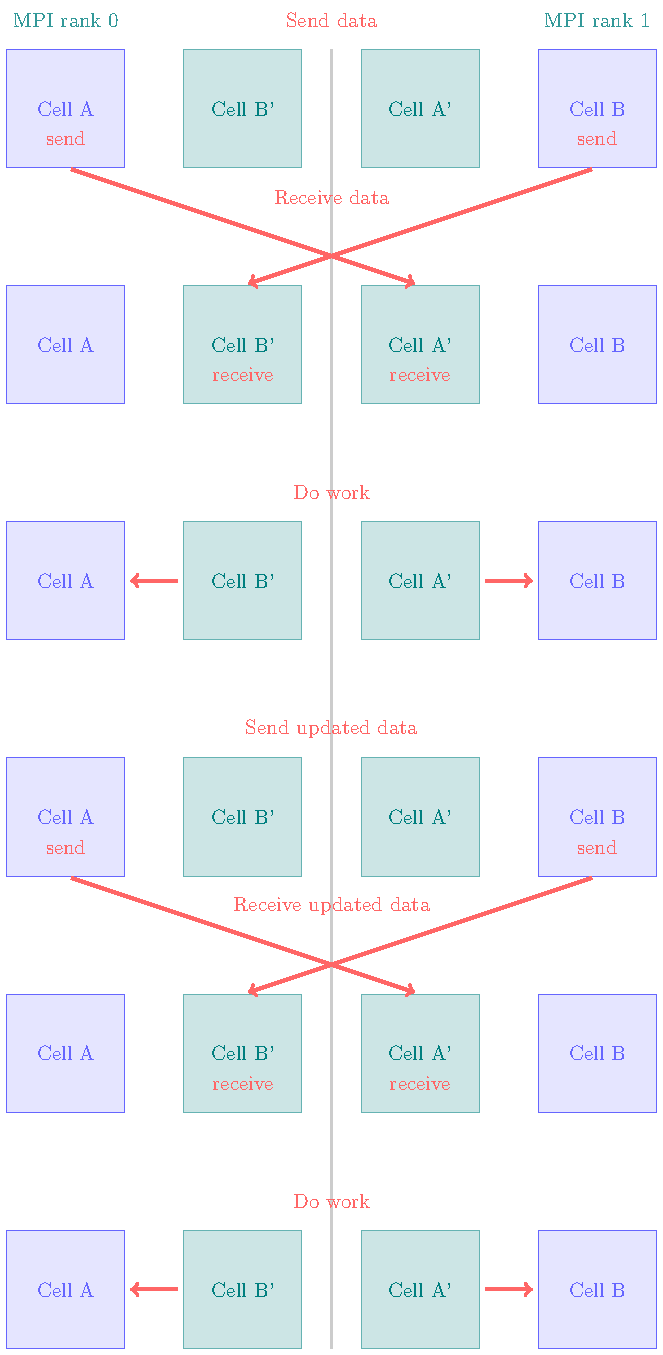
\includegraphics[height=.75\textheight]{figures/Meshless/repeated_mpi_comm.pdf}
 \caption{
Illustration of how the communication logic is set up in \swift for situations where updated data
of
\lingo{foreign} cells are necessary. It starts with \lingo{real} cells $A$ and $B$ sending their
current state of data to their \lingo{foreign} counterparts, $A'$ and $B'$, respectively. Once $A'$
and $B'$ have received the data, the individual ranks can proceed with the work necessary for their
\lingo{real} cells $A$ and $B$. In the depicted situation, cells $A$ and $B$ then undergo a
second interaction with each other, and hence the \lingo{foreign} cells $A'$ and $B'$ need to be
updated to the current state of $A$ and $B$. To this end, the cells $A$ and $B$ once again send
their data, and the second interaction can take place once $A'$ and $B'$ have received the data.
Note that \lingo{foreign} cells are never updated on foreign ranks, only \lingo{real} cells are
updated. \lingo{Foreign} cells' only purpose is to make the necessary data available for other
\lingo{real} cells on their respective \lingo{ranks}. This restriction allows to never need to send
data back from foreign cells $A'$ and $B'$ to their \lingo{real} counterparts $A$ and $B$. Also
note that despite what this sketch might suggest, the send and receive operations (and tasks) of
cells do not need to occur simultaneously, and in general will not be executed concurrently.
}
 \label{fig:mpi-comm-repeated}
\end{figure}



MPI provides developers with a programming interface to transfer data between individual
\lingo{ranks}, or collectively among all \lingo{ranks} involved in a process. The communications
between individual \lingo{ranks} consist of explicit calls to send and to receive certain data. If
for example the MPI \lingo{rank} 0 needed to send data to MPI \lingo{rank} 1, \lingo{rank} 0 would
send a message addressed to \lingo{rank} 1, while \lingo{rank} 1 would need to expect and receive
that message. Traditionally, this data exchange would occur with so-called ``\lingo{blocking}'' or
``\lingo{synchronous}'' calls to the send and receive functions. The message is sent and received
only when both \lingo{ranks} arrive at the point where a message needs to be exchanged, and then
both \lingo{ranks} would proceed with their respective work. Until each \lingo{rank} involved in
the communication reaches the synchronization point at which the message is exchanged, the others
are blocked from proceeding any further, and wait for all \lingo{ranks} involved in this
communication to reach the synchronization point. However, the task-based parallelism of \swift
allows for the communications to be completely \lingo{asynchronous}: Any \lingo{rank} can send the
data it needs to send whenever it is ready to send it, and then proceed to work on other tasks
without waiting at a synchronization point until the message is received. Conversely, the receiving
\lingo{ranks} can keep checking whether the necessary data has arrived. While the data hasn't been
received yet, the receiving \lingo{rank} can also simply proceed to work on other tasks without
wasting time waiting at synchronization points, and check again whether data has arrived after it
completed a different task.


More concretely, the data that needs to be communicated consists of data contained within cells.
This includes all particles within a cell, as well as other cell data such as the minimal time step
size within the cell. A local copy of cells assigned to some given MPI \lingo{rank}'s domain is
created on the \lingo{ranks} which require that particular cell's data. These cells are called
``\lingo{foreign}'' cells. The required communications then consist of transmitting the up-to-date
data from the ``\lingo{real}'' cell into the corresponding \lingo{foreign} cell. This way, the
other \lingo{ranks} can do the necessary work as if the \lingo{foreign} cell is a normal one and
part of their domain, with the exception that they don't need to do work on the particles in the
\lingo{foreign} cell itself. The actual work on the \lingo{foreign} cells is performed by the
\lingo{rank} where their corresponding \lingo{real} counterpart situated. Figure~\ref{fig:mpi-comm}
shows the working principle how two cells $A$ and $B$ first get assigned to two different MPI
\lingo{ranks} during the domain decomposition, and a \lingo{foreign} counterpart cell $A'$ and $B'$
is created on the other \lingo{rank}, respectively. It then goes on to show how a first
communication takes place: \lingo{Real} cells $A$ and $B$ send their data to the foreign
counterparts $A'$ and $B'$, respectively. The \lingo{foreign} cells $A'$ and $B'$ receive data when
the corresponding receive tasks are executed. Finally the work can proceed, and the ``real'' cells
$A$ and $B$ can updated correctly.

In cases where several updates of \lingo{foreign} cells are required during a single simulation
step, the updated data of the \lingo{real} cells is being sent and received again. Let us stress
once again that data of \lingo{foreign} cells is never updated by the ranks where the cells are
\lingo{foreign}, they are merely used to make necessary data for the \lingo{real} cells of the
\lingo{rank} available. \lingo{Foreign} cells are only updated by receiving the updated data from
the \lingo{real} cells. While this may seem like a harsh restriction, it allows to make the
algorithm work without ever needing to send data back from \lingo{foreign} cells to their
\lingo{real} counterparts. So in total, it reduces the required number of communications.
Figure~\ref{fig:mpi-comm-repeated} shows how the algorithm works when several updates and hence MPI
communications are required.
















%--------------------------------------------------------
\subsubsection{MPI Tasks}
%--------------------------------------------------------



\begin{figure}
 \centering
 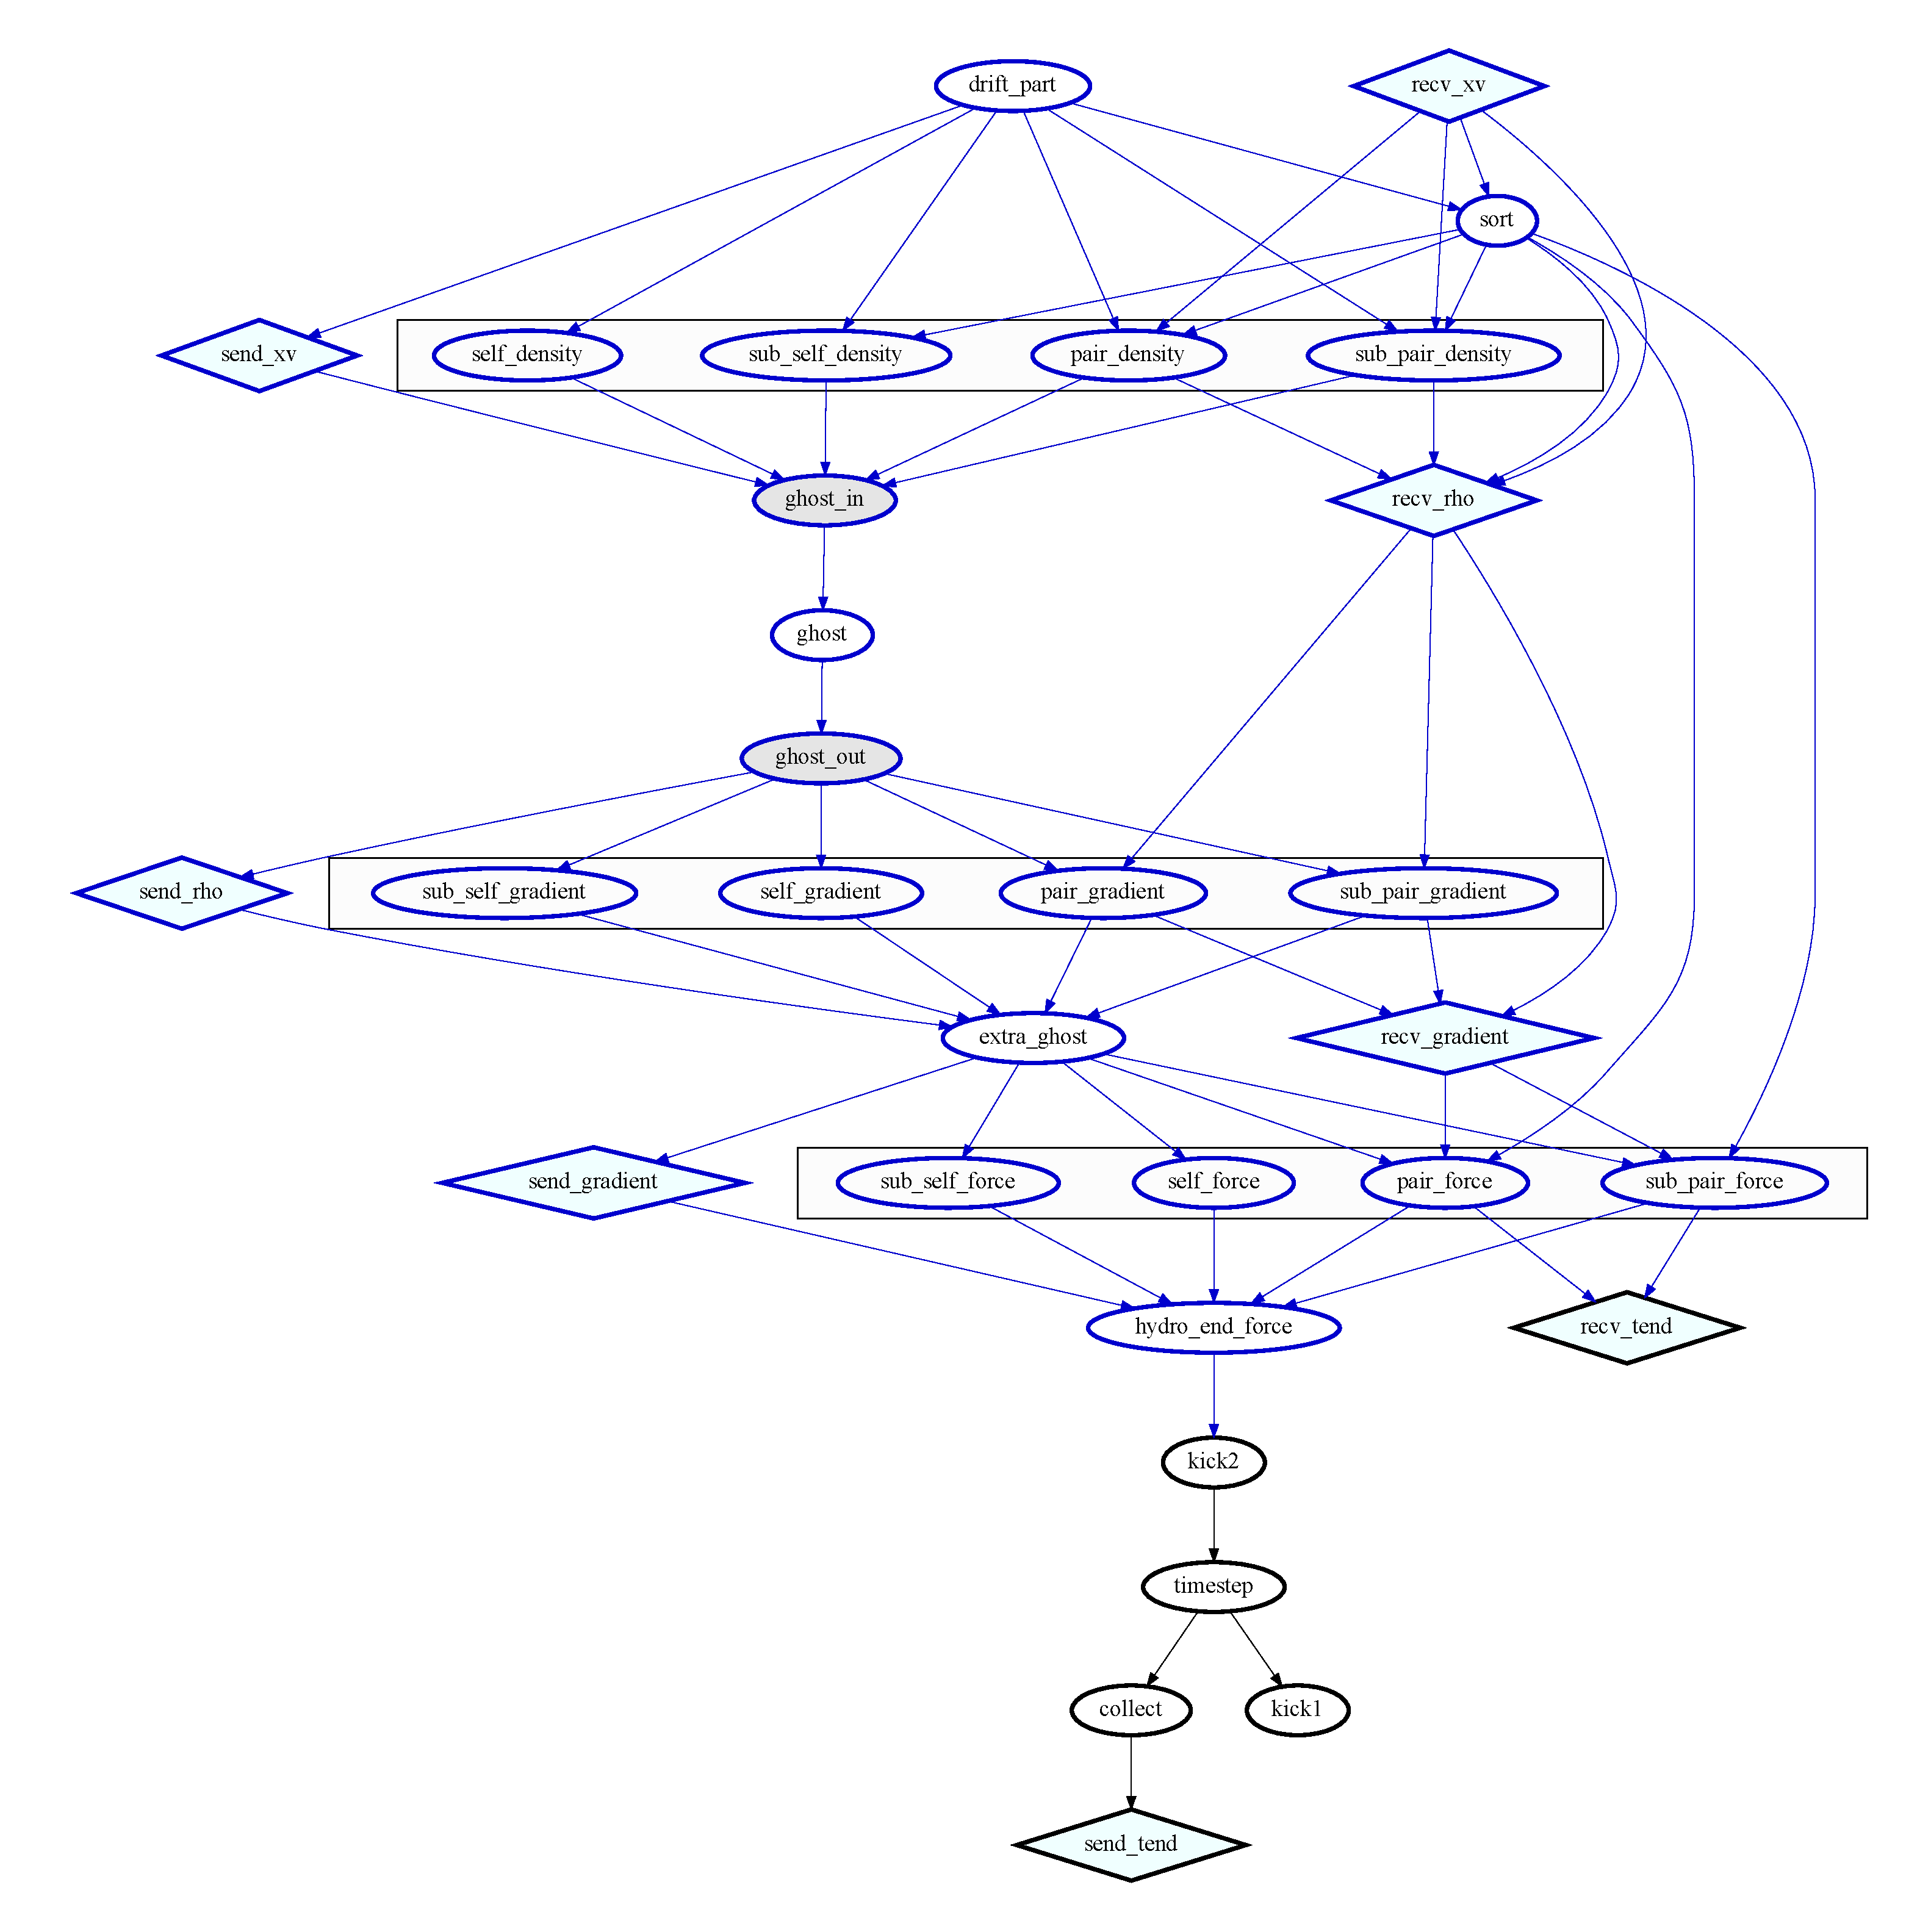
\includegraphics[width=\textwidth]{figures/Meshless/tasks_hydro_only.pdf}
 \caption{
The full dependency graph required for finite volume particle hydrodynamics with \swift and MPI.
Before each
interaction loop (density, gradient, and force) an updated state of foreign cells is necessary.
After the timestep tasks have finished, an additional update with the current minimal time step
sizes inside the foreign cells is necessary to facilitate the correct task activation at the
beginning of the subsequent simulation step.
}
 \label{fig:dependency-graph-hydro}
\end{figure}


With the basic working principle of asynchronous MPI communications having been discussed, we can
now proceed to add the corresponding required tasks and dependencies to the dependency graph for
finite volume particle hydrodynamics in \swift, whose final form is shown in
Figure~\ref{fig:dependency-graph-hydro}. The \lingo{foreign} cells need to be up-to-date before each
particle-particle interaction, i.e. they need to receive data before the \lingo{density} tasks are
run, then again before the \lingo{gradient} tasks are run, and finally again before the fluxes are
exchanged in \lingo{force} tasks. The first receiving task on the graph, called
``\lingo{recv\_xv}'', is the task that is used to receive the data from the corresponding
\lingo{real} cell before the neighbor search (\lingo{density}) interaction can take place. It is
named with the suffix ``\lingo{xv}'' as its purpose is primarily to receive the current positions
and velocities of particles. The particles are first drifted in the corresponding \lingo{real}
cell before the data is sent, hence there will be a dependency from the \lingo{drift\_part} to the
\lingo{send\_xv} tasks, and the data \lingo{recv\_xv} tasks receive will contain particles drifted
to the correct time.  Once the data is received, the particles are sorted along each neighboring
cells' axes for an optimized access to particles during interactions, as was previously mentioned.
(Note that this doesn't modify any particle values, but only creates lists of sorted particles for
the cells). The \lingo{send\_xv} task has an outgoing dependency to the first task after the
interaction loop, which in this case is the \lingo{ghost\_in} task. The reason this dependency is
needed is because we can't allow the cell to be updated any further before the data has been sent,
which is what this dependency ensures. Explicitly, this dependency ensures that the
\lingo{ghost\_in} tasks can't be executed before the \lingo{send\_xv} task is finished.

On the receiving side, dependencies between \lingo{recv\_xv} and \lingo{pair}-type tasks of the
\lingo{density} loop are necessary: The interactions must not take place before the data has
arrived. Recall that actual work is never done on \lingo{foreign} cells, which are the only cell
types that have an associated \lingo{receive}-type task. So cells which have \lingo{receive}-type
tasks will never have \lingo{self}-type tasks, which are the ones that interact particles within a
cell with each other. Therefore no dependencies between \lingo{receive}-type tasks and
\lingo{self}-type tasks are necessary. For the same reason, only dependencies from \lingo{pair}-type
(and \lingo{sub-pair}) type tasks are required for the subsequent \lingo{receive}-type task, which
is the \lingo{recv\_density} task. Additionally, it is necessary to add a dependency between two
\lingo{receive}-type tasks: MPI doesn't guarantee in which order messages will arrive. Allowing two
\lingo{receive}-type tasks of a single \lingo{foreign} cell to be ready for execution concurrently
permits the message that should be arriving later to be received first. The remaining message, which
should have arrived first, will then overwrite the already received message's data with data which
is incorrect at that point. Therefore it is necessary to forbid \lingo{receive}-type tasks to run
concurrently, which is achieved by adding a dependency between them. The same logic applies to the
\lingo{send}-type and \lingo{receive}-type tasks in the subsequent particle-particle interaction
loops.

To summarize, the required sending and receiving types of tasks for a hydrodynamics step are as
follows:

On the sending side:

\begin{itemize}
 \item After drifting particles, send over the updated particle positions using \lingo{send\_xv}.
 \item After doing the neighbor search loop with the \lingo{density} tasks, send the updated
particle data over for the computation of gradients with the \lingo{send\_rho} tasks before you
continue modifying the particle data.
 \item After finishing the gradient computations in the \lingo{gradient} tasks, send the updated
particle data over with the \lingo{send\_gradient} tasks for the computation of fluxes before you
continue modifying the particle data.
\end{itemize}

On the receiving side:

\begin{itemize}
 \item Before doing a neighbor search loop, receive the updated particle positions using
\lingo{recv\_xv} and sort the particles.
 \item Before doing the gradient loop, receive the updated particle ``densities'' with
\lingo{recv\_rho}.
 \item Before doing the flux exchange (\lingo{force}) loop, receive the updated particle
gradients.
\end{itemize}


Finally, once the new time step sizes for particles have been computed with the \lingo{timestep}
tasks once the time integration in this simulation step has been completed, a final update needs to
take place. The \lingo{foreign} cells need to have the correct cell information available which is
required for the task activation process in the subsequent simulation step. Concretely, this is the
smallest time step size contained within the cell, and the last time the cell was updated. Rather
than sending all particle data again, it suffices to only send this cell metadata. The full updated
particle data will be sent over with the \lingo{send\_xv} task at the beginning of the next
simulation step anyway. The cell metadata is being sent using the \lingo{send\_tend} tasks, and
correspondingly received by the \lingo{recv\_tend} tasks.


























